\documentclass[12pt]{article}
\usepackage[margin=1in]{geometry} 
\usepackage{amsmath,amsthm,amssymb,amsfonts}
\usepackage{graphicx}
\usepackage{listings}
\usepackage{enumitem}
\usepackage{amsmath}
\usepackage{tikz}
\usepackage{stmaryrd}

\newcommand{\N}{\mathbb{N}}
\newcommand{\Z}{\mathbb{Z}}
 
\newenvironment{problem}[2][Problem]{\begin{trivlist}
\item[\hskip \labelsep {\bfseries #1}\hskip \labelsep {\bfseries #2.}]}{\end{trivlist}}
\setlength{\parskip}{1em}

\begin{document}
\title{COMP.3040 Homework 4}

\maketitle

\begin{problem}{3.1}
\end{problem}
\begin{enumerate}
	\item[(a)] ~

		\tikzset{every picture/.style={line width=0.75pt}} %set default line width to 0.75pt        
		
		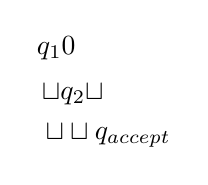
\begin{tikzpicture}[x=0.75pt,y=0.75pt,yscale=-1,xscale=1]
		%uncomment if require: \path (0,95); %set diagram left start at 0, and has height of 95
		
		% Text Node
		\draw (287,34) node  [align=left] {$\displaystyle q_{1} 0$};
		% Text Node
		\draw (295,56) node  [align=left] {$\displaystyle \sqcup q_{2} \sqcup $};
		% Text Node
		\draw (312,76) node  [align=left] {$\displaystyle \sqcup \sqcup q_{accept}$};
		
		\end{tikzpicture}

	\item[(c)]~

		\tikzset{every picture/.style={line width=0.75pt}} %set default line width to 0.75pt        
		
		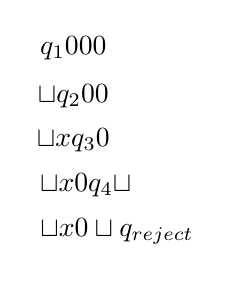
\begin{tikzpicture}[x=0.75pt,y=0.75pt,yscale=-1,xscale=1]
		%uncomment if require: \path (0,166); %set diagram left start at 0, and has height of 166
		
		% Text Node
		\draw (211,50) node  [align=left] {$\displaystyle q_{1} 000$};
		% Text Node
		\draw (211,73) node  [align=left] {$\displaystyle \sqcup q_{2} 00$};
		% Text Node
		\draw (211,94) node  [align=left] {$\displaystyle \sqcup xq_{3} 0$};
		% Text Node
		\draw (217,116) node  [align=left] {$\displaystyle \sqcup x0q_{4} \sqcup $};
		% Text Node
		\draw (232,138) node  [align=left] {$\displaystyle \sqcup x0\sqcup q_{reject}$};
		
		\end{tikzpicture}

	\item[(d)]~

		\tikzset{every picture/.style={line width=0.75pt}} %set default line width to 0.75pt        
		
		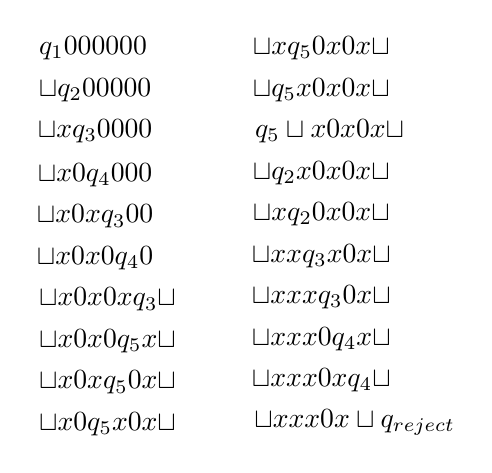
\begin{tikzpicture}[x=0.75pt,y=0.75pt,yscale=-1,xscale=1]
		%uncomment if require: \path (0,252.42856979370117); %set diagram left start at 0, and has height of 252.42856979370117
		
		% Text Node
		\draw (223,35) node  [align=left] {$\displaystyle q_{1} 000000$};
		% Text Node
		\draw (224,55) node  [align=left] {$\displaystyle \sqcup q_{2} 00000$};
		% Text Node
		\draw (224,75) node  [align=left] {$\displaystyle \sqcup xq_{3} 0000$};
		% Text Node
		\draw (224,96) node  [align=left] {$\displaystyle \sqcup x0q_{4} 000$};
		% Text Node
		\draw (224,116) node  [align=left] {$\displaystyle \sqcup x0xq_{3} 00$};
		% Text Node
		\draw (224,136) node  [align=left] {$\displaystyle \sqcup x0x0q_{4} 0$};
		% Text Node
		\draw (230,156) node  [align=left] {$\displaystyle \sqcup x0x0xq_{3} \sqcup $};
		% Text Node
		\draw (230,176) node  [align=left] {$\displaystyle \sqcup x0x0q_{5} x \sqcup $};
		% Text Node
		\draw (230,196) node  [align=left] {$\displaystyle \sqcup x0xq_{5} 0x \sqcup $};
		% Text Node
		\draw (230,216) node  [align=left] {$\displaystyle \sqcup x0q_{5} x0x \sqcup $};
		% Text Node
		\draw (333,35) node  [align=left] {$\displaystyle \sqcup xq_{5} 0x0x \sqcup $};
		% Text Node
		\draw (333,55) node  [align=left] {$\displaystyle \sqcup q_{5} x0x0x \sqcup $};
		% Text Node
		\draw (337,75) node  [align=left] {$\displaystyle q_{5} \sqcup x0x0x \sqcup $};
		% Text Node
		\draw (333,95) node  [align=left] {$\displaystyle \sqcup q_{2} x0x0x \sqcup $};
		% Text Node
		\draw (333,115) node  [align=left] {$\displaystyle \sqcup xq_{2} 0x0x \sqcup $};
		% Text Node
		\draw (333,135) node  [align=left] {$\displaystyle \sqcup xxq_{3} x0x \sqcup $};
		% Text Node
		\draw (333,155) node  [align=left] {$\displaystyle \sqcup xxxq_{3} 0x \sqcup $};
		% Text Node
		\draw (333,175) node  [align=left] {$\displaystyle \sqcup xxx0q_{4} x \sqcup $};
		% Text Node
		\draw (333,195) node  [align=left] {$\displaystyle \sqcup xxx0xq_{4} \sqcup $};
		% Text Node
		\draw (349,215) node  [align=left] {$\displaystyle \sqcup xxx0x \sqcup q_{reject}$};
		
		\end{tikzpicture}

\end{enumerate}
Input string 00000000: 	\\

	\tikzset{every picture/.style={line width=0.75pt}} %set default line width to 0.75pt        
	
	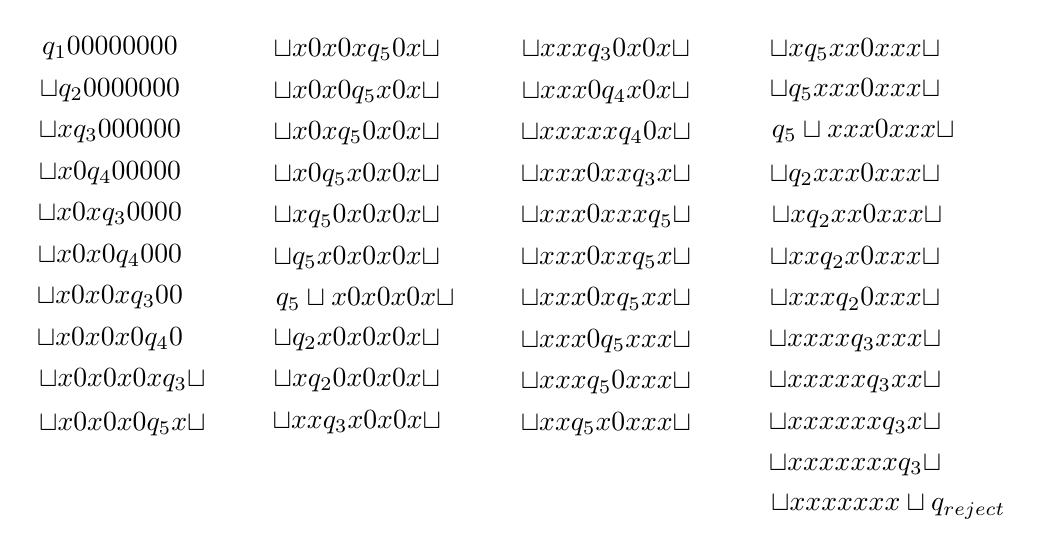
\begin{tikzpicture}[x=0.75pt,y=0.75pt,yscale=-1,xscale=1]
	%uncomment if require: \path (0,284.42857360839844); %set diagram left start at 0, and has height of 284.42857360839844
	
	% Text Node
	\draw (122,35) node  [align=left] {$\displaystyle q_{1} 00000000$};
	% Text Node
	\draw (122,55) node  [align=left] {$\displaystyle \sqcup q_{2} 0000000$};
	% Text Node
	\draw (122,75) node  [align=left] {$\displaystyle \sqcup xq_{3} 000000$};
	% Text Node
	\draw (122,95) node  [align=left] {$\displaystyle \sqcup x0q_{4} 00000$};
	% Text Node
	\draw (122,115) node  [align=left] {$\displaystyle \sqcup x0xq_{3} 0000$};
	% Text Node
	\draw (122,135) node  [align=left] {$\displaystyle \sqcup x0x 0q_{4} 000$};
	% Text Node
	\draw (122,155) node  [align=left] {$\displaystyle \sqcup x0x 0xq_{3} 00$};
	% Text Node
	\draw (122,175) node  [align=left] {$\displaystyle \sqcup x0x 0x0q_{4} 0$};
	% Text Node
	\draw (128,195) node  [align=left] {$\displaystyle \sqcup x0x 0x0xq_{3} \sqcup $};
	% Text Node
	\draw (128,216) node  [align=left] {$\displaystyle \sqcup x0x 0x0q_{5} x \sqcup $};
	% Text Node
	\draw (241,36) node  [align=left] {$\displaystyle \sqcup x0x 0xq_{5} 0x \sqcup $};
	% Text Node
	\draw (245,156) node  [align=left] {$\displaystyle q_{5} \sqcup x0x 0x0 x \sqcup $};
	% Text Node
	\draw (241,136) node  [align=left] {$\displaystyle \sqcup q_{5} x0x 0x0 x \sqcup $};
	% Text Node
	\draw (241,116) node  [align=left] {$\displaystyle \sqcup xq_{5} 0x 0x0x \sqcup $};
	% Text Node
	\draw (241,96) node  [align=left] {$\displaystyle \sqcup x0q_{5} x 0x0x \sqcup $};
	% Text Node
	\draw (241,76) node  [align=left] {$\displaystyle \sqcup x0xq_{5} 0x0x \sqcup $};
	% Text Node
	\draw (241,56) node  [align=left] {$\displaystyle \sqcup x0x 0q_{5} x0x \sqcup $};
	% Text Node
	\draw (241,175) node  [align=left] {$\displaystyle \sqcup q_{2} x0x 0x0 x \sqcup $};
	% Text Node
	\draw (241,195) node  [align=left] {$\displaystyle \sqcup xq_{2} 0x 0x0 x \sqcup $};
	% Text Node
	\draw (241,215) node  [align=left] {$\displaystyle \sqcup xxq_{3} x 0x0 x \sqcup $};
	% Text Node
	\draw (361,36) node  [align=left] {$\displaystyle \sqcup xxxq_{3} 0x0 x \sqcup $};
	% Text Node
	\draw (361,56) node  [align=left] {$\displaystyle \sqcup xxx0q_{4} x0 x \sqcup $};
	% Text Node
	\draw (361,76) node  [align=left] {$\displaystyle \sqcup xxxxxq_{4} 0 x \sqcup $};
	% Text Node
	\draw (361,96) node  [align=left] {$\displaystyle \sqcup xxx0xxq_{3} x \sqcup $};
	% Text Node
	\draw (361,116) node  [align=left] {$\displaystyle \sqcup xxx0xxxq_{5} \sqcup $};
	% Text Node
	\draw (361,136) node  [align=left] {$\displaystyle \sqcup xxx0xxq_{5} x\sqcup $};
	% Text Node
	\draw (481,55) node  [align=left] {$\displaystyle \sqcup q_{5} xxx0xxx\sqcup $};
	% Text Node
	\draw (481,36) node  [align=left] {$\displaystyle \sqcup xq_{5} xx0xxx\sqcup $};
	% Text Node
	\draw (361,216) node  [align=left] {$\displaystyle \sqcup xxq_{5} x0xxx\sqcup $};
	% Text Node
	\draw (361,196) node  [align=left] {$\displaystyle \sqcup xxxq_{5} 0xxx\sqcup $};
	% Text Node
	\draw (361,176) node  [align=left] {$\displaystyle \sqcup xxx0q_{5} xxx\sqcup $};
	% Text Node
	\draw (361,156) node  [align=left] {$\displaystyle \sqcup xxx0xq_{5} xx\sqcup $};
	% Text Node
	\draw (485,75) node  [align=left] {$\displaystyle q_{5} \sqcup xxx0xxx\sqcup $};
	% Text Node
	\draw (481,96) node  [align=left] {$\displaystyle \sqcup q_{2} xxx0xxx\sqcup $};
	% Text Node
	\draw (482,116) node  [align=left] {$\displaystyle \sqcup xq_{2} xx0xxx\sqcup $};
	% Text Node
	\draw (481,236) node  [align=left] {$\displaystyle \sqcup xxxxxxxq_{3} \sqcup $};
	% Text Node
	\draw (481,176) node  [align=left] {$\displaystyle \sqcup xxxxq_{3} xxx\sqcup $};
	% Text Node
	\draw (481,216) node  [align=left] {$\displaystyle \sqcup xxxxxxq_{3} x\sqcup $};
	% Text Node
	\draw (481,196) node  [align=left] {$\displaystyle \sqcup xxxxxq_{3} xx\sqcup $};
	% Text Node
	\draw (481,156) node  [align=left] {$\displaystyle \sqcup xxxq_{2} 0xxx\sqcup $};
	% Text Node
	\draw (481,136) node  [align=left] {$\displaystyle \sqcup xxq_{2} x0xxx\sqcup $};
	% Text Node
	\draw (497,256) node  [align=left] {$\displaystyle \sqcup xxxxxxx\sqcup q_{reject}$};
	
	\end{tikzpicture}


\begin{problem}{3.2}
\end{problem}
\begin{enumerate}
	\item[(b)]~

		\tikzset{every picture/.style={line width=0.75pt}} %set default line width to 0.75pt        
		
		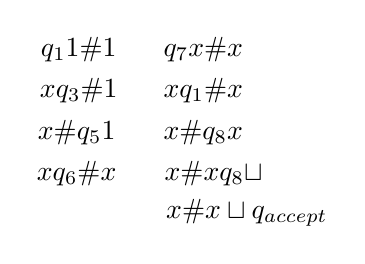
\begin{tikzpicture}[x=0.75pt,y=0.75pt,yscale=-1,xscale=1]
		%uncomment if require: \path (0,235.42855834960938); %set diagram left start at 0, and has height of 235.42855834960938
		
		% Text Node
		\draw (330,35) node  [align=left] {$\displaystyle q_{1} 1\#1$};
		% Text Node
		\draw (330,55) node  [align=left] {$\displaystyle xq_{3} \#1$};
		% Text Node
		\draw (329,75) node  [align=left] {$\displaystyle x \#q_{5} 1$};
		% Text Node
		\draw (329,95) node  [align=left] {$\displaystyle xq_{6} \#x$};
		% Text Node
		\draw (390,35) node  [align=left] {$\displaystyle q_{7} x\#x$};
		% Text Node
		\draw (390,55) node  [align=left] {$\displaystyle xq_{1} \#x$};
		% Text Node
		\draw (390,75) node  [align=left] {$\displaystyle x\#q_{8} x$};
		% Text Node
		\draw (395,95) node  [align=left] {$\displaystyle x\# xq_{8} \sqcup $};
		% Text Node
		\draw (411,114) node  [align=left] {$\displaystyle x\# x\sqcup q_{accept}$};
		
		\end{tikzpicture}

	\item[(c)]~

		\tikzset{every picture/.style={line width=0.75pt}} %set default line width to 0.75pt        
		
		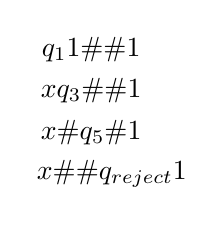
\begin{tikzpicture}[x=0.75pt,y=0.75pt,yscale=-1,xscale=1]
		%uncomment if require: \path (0,132.5); %set diagram left start at 0, and has height of 132.5
		
		% Text Node
		\draw (324,35) node  [align=left] {$\displaystyle q_{1} 1\#\#1$};
		% Text Node
		\draw (324,55) node  [align=left] {$\displaystyle xq_{3} \#\#1$};
		% Text Node
		\draw (324,75) node  [align=left] {$\displaystyle x\#q_{5} \#1$};
		% Text Node
		\draw (334,95) node  [align=left] {$\displaystyle x\#\#q_{reject} 1$};
		
		\end{tikzpicture}

	\item[(d)]~

		\tikzset{every picture/.style={line width=0.75pt}} %set default line width to 0.75pt        
		
		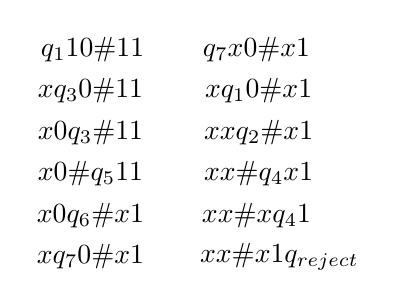
\begin{tikzpicture}[x=0.75pt,y=0.75pt,yscale=-1,xscale=1]
		%uncomment if require: \path (0,179); %set diagram left start at 0, and has height of 179
		
		% Text Node
		\draw (339,35) node  [align=left] {$\displaystyle q_{1} 10\#11$};
		% Text Node
		\draw (338,55) node  [align=left] {$\displaystyle xq_{3} 0\#11$};
		% Text Node
		\draw (338,75) node  [align=left] {$\displaystyle x0q_{3} \#11$};
		% Text Node
		\draw (338,95) node  [align=left] {$\displaystyle x0\#q_{5} 11$};
		% Text Node
		\draw (338,115) node  [align=left] {$\displaystyle x0q_{6} \#x1$};
		% Text Node
		\draw (338,135) node  [align=left] {$\displaystyle xq_{7} 0\#x1$};
		% Text Node
		\draw (418,35) node  [align=left] {$\displaystyle q_{7} x0\#x1$};
		% Text Node
		\draw (419,55) node  [align=left] {$\displaystyle xq_{1} 0\#x1$};
		% Text Node
		\draw (419,75) node  [align=left] {$\displaystyle xxq_{2} \#x1$};
		% Text Node
		\draw (419,95) node  [align=left] {$\displaystyle xx\#q_{4} x1$};
		% Text Node
		\draw (418,115) node  [align=left] {$\displaystyle xx\#xq_{4} 1$};
		% Text Node
		\draw (429,135) node  [align=left] {$\displaystyle xx\#x1q_{reject}$};
		
		\end{tikzpicture}

	\item[(e)]~

		\tikzset{every picture/.style={line width=0.75pt}} %set default line width to 0.75pt        
		
		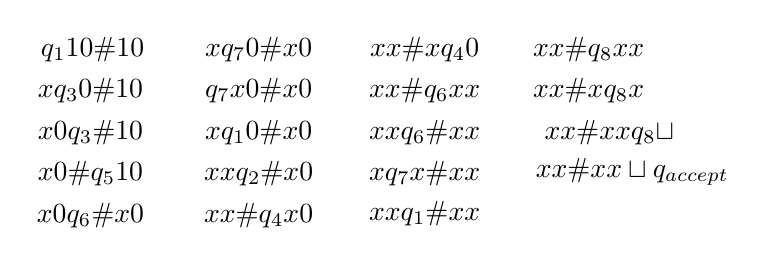
\begin{tikzpicture}[x=0.75pt,y=0.75pt,yscale=-1,xscale=1]
		%uncomment if require: \path (0,208); %set diagram left start at 0, and has height of 208
		
		% Text Node
		\draw (199,35) node  [align=left] {$\displaystyle q_{1} 10\#10$};
		% Text Node
		\draw (198,55) node  [align=left] {$\displaystyle xq_{3} 0\#10$};
		% Text Node
		\draw (198,75) node  [align=left] {$\displaystyle x0q_{3} \#10$};
		% Text Node
		\draw (198,95) node  [align=left] {$\displaystyle x0\#q_{5} 10$};
		% Text Node
		\draw (198,115) node  [align=left] {$\displaystyle x0q_{6} \#x0$};
		% Text Node
		\draw (279,35) node  [align=left] {$\displaystyle xq_{7} 0\#x0$};
		% Text Node
		\draw (279,55) node  [align=left] {$\displaystyle q_{7} x0\#x0$};
		% Text Node
		\draw (279,75) node  [align=left] {$\displaystyle xq_{1} 0\#x0$};
		% Text Node
		\draw (279,95) node  [align=left] {$\displaystyle xxq_{2} \#x0$};
		% Text Node
		\draw (279,115) node  [align=left] {$\displaystyle xx\#q_{4} x0$};
		% Text Node
		\draw (359,35) node  [align=left] {$\displaystyle xx\#xq_{4} 0$};
		% Text Node
		\draw (359,55) node  [align=left] {$\displaystyle xx\#q_{6} xx$};
		% Text Node
		\draw (359,75) node  [align=left] {$\displaystyle xxq_{6} \#xx$};
		% Text Node
		\draw (359,95) node  [align=left] {$\displaystyle xq_{7} x\#xx$};
		% Text Node
		\draw (359,114) node  [align=left] {$\displaystyle xxq_{1} \#xx$};
		% Text Node
		\draw (438,35) node  [align=left] {$\displaystyle xx\#q_{8} xx$};
		% Text Node
		\draw (438,55) node  [align=left] {$\displaystyle xx\#xq_{8} x$};
		% Text Node
		\draw (448,75) node  [align=left] {$\displaystyle xx\#xxq_{8} \sqcup $};
		% Text Node
		\draw (459,94) node  [align=left] {$\displaystyle xx\#xx\sqcup q_{accept}$};
		
		\end{tikzpicture}

\end{enumerate}
Input string 01100\#01100: 	\\

	\tikzset{every picture/.style={line width=0.75pt}} %set default line width to 0.75pt        
	
	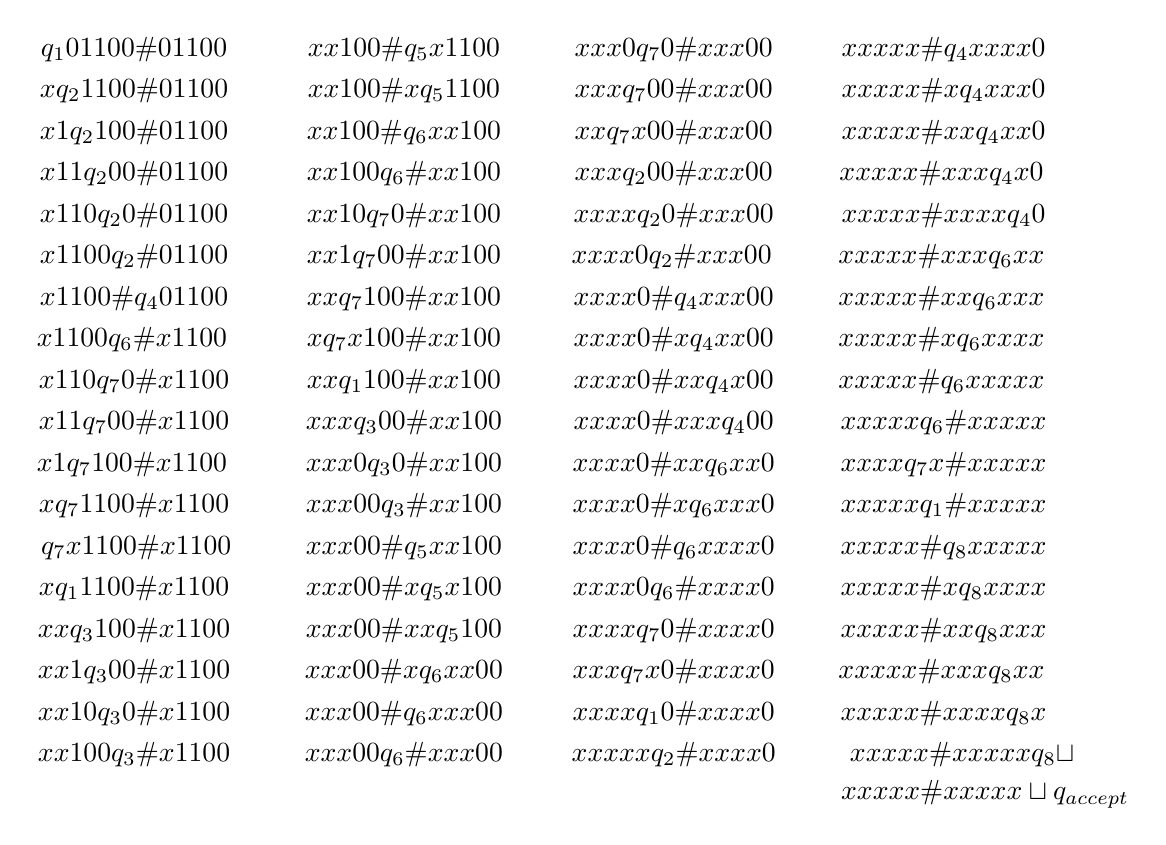
\begin{tikzpicture}[x=0.75pt,y=0.75pt,yscale=-1,xscale=1]
	%uncomment if require: \path (0,441.36607360839844); %set diagram left start at 0, and has height of 441.36607360839844
	
	% Text Node
	\draw (134,35) node  [align=left] {$\displaystyle q_{1} 01100\#01100$};
	% Text Node
	\draw (134,55) node  [align=left] {$\displaystyle xq_{2} 1100\#01100$};
	% Text Node
	\draw (134,75) node  [align=left] {$\displaystyle x1q_{2} 100\#01100$};
	% Text Node
	\draw (134,95) node  [align=left] {$\displaystyle x11q_{2} 00\#01100$};
	% Text Node
	\draw (134,135) node  [align=left] {$\displaystyle x1100q_{2} \#01100$};
	% Text Node
	\draw (134,115) node  [align=left] {$\displaystyle x110q_{2} 0\#01100$};
	% Text Node
	\draw (134,155) node  [align=left] {$\displaystyle x1100 \#q_{4} 01100$};
	% Text Node
	\draw (133,175) node  [align=left] {$\displaystyle x1100q_{6} \#x 1100$};
	% Text Node
	\draw (134,195) node  [align=left] {$\displaystyle x110q_{7} 0\#x 1100$};
	% Text Node
	\draw (134,215) node  [align=left] {$\displaystyle x11q_{7} 00\#x 1100$};
	% Text Node
	\draw (134,255) node  [align=left] {$\displaystyle xq_{7} 1100\#x 1100$};
	% Text Node
	\draw (133,235) node  [align=left] {$\displaystyle x1q_{7} 100\#x 1100$};
	% Text Node
	\draw (135,275) node  [align=left] {$\displaystyle q_{7} x1100\#x 1100$};
	% Text Node
	\draw (134,295) node  [align=left] {$\displaystyle xq_{1} 1100\#x 1100$};
	% Text Node
	\draw (134,315) node  [align=left] {$\displaystyle xxq_{3} 100\#x 1100$};
	% Text Node
	\draw (134,335) node  [align=left] {$\displaystyle xx1q_{3} 00\#x 1100$};
	% Text Node
	\draw (134,375) node  [align=left] {$\displaystyle xx100q_{3} \#x 1100$};
	% Text Node
	\draw (134,355) node  [align=left] {$\displaystyle xx10q_{3} 0\#x 1100$};
	% Text Node
	\draw (264,35) node  [align=left] {$\displaystyle xx100\#q_{5} x 1100$};
	% Text Node
	\draw (264,55) node  [align=left] {$\displaystyle xx100\#xq_{5} 1100$};
	% Text Node
	\draw (264,75) node  [align=left] {$\displaystyle xx100\#q_{6} xx100$};
	% Text Node
	\draw (264,95) node  [align=left] {$\displaystyle xx100q_{6} \#xx100$};
	% Text Node
	\draw (264,115) node  [align=left] {$\displaystyle xx10q_{7} 0\#xx100$};
	% Text Node
	\draw (264,135) node  [align=left] {$\displaystyle xx1q_{7} 00\#xx100$};
	% Text Node
	\draw (264,155) node  [align=left] {$\displaystyle xxq_{7} 100\#xx100$};
	% Text Node
	\draw (264,175) node  [align=left] {$\displaystyle xq_{7} x100\#xx100$};
	% Text Node
	\draw (264,195) node  [align=left] {$\displaystyle xxq_{1} 100\#xx100$};
	% Text Node
	\draw (264,215) node  [align=left] {$\displaystyle xxxq_{3} 00\#xx100$};
	% Text Node
	\draw (264,235) node  [align=left] {$\displaystyle xxx0q_{3} 0\#xx100$};
	% Text Node
	\draw (264,255) node  [align=left] {$\displaystyle xxx00q_{3} \#xx100$};
	% Text Node
	\draw (264,275) node  [align=left] {$\displaystyle xxx00\#q_{5} xx100$};
	% Text Node
	\draw (264,295) node  [align=left] {$\displaystyle xxx00\#xq_{5} x100$};
	% Text Node
	\draw (264,315) node  [align=left] {$\displaystyle xxx00\#xxq_{5} 100$};
	% Text Node
	\draw (264,335) node  [align=left] {$\displaystyle xxx00\#xq_{6} xx00$};
	% Text Node
	\draw (264,355) node  [align=left] {$\displaystyle xxx00\#q_{6} xxx00$};
	% Text Node
	\draw (264,375) node  [align=left] {$\displaystyle xxx00q_{6} \#xxx00$};
	% Text Node
	\draw (394,35) node  [align=left] {$\displaystyle xxx0q_{7} 0\#xxx00$};
	% Text Node
	\draw (394,55) node  [align=left] {$\displaystyle xxxq_{7} 0 0\#xxx00$};
	% Text Node
	\draw (394,75) node  [align=left] {$\displaystyle xxq_{7} x 0 0\#xxx00$};
	% Text Node
	\draw (394,95) node  [align=left] {$\displaystyle xxxq_{2} 0 0\#xxx00$};
	% Text Node
	\draw (394,115) node  [align=left] {$\displaystyle xxxxq_{2} 0\#xxx00$};
	% Text Node
	\draw (393,135) node  [align=left] {$\displaystyle xxxx0q_{2} \#xxx00$};
	% Text Node
	\draw (394,155) node  [align=left] {$\displaystyle xxxx0\#q_{4} xxx00$};
	% Text Node
	\draw (394,175) node  [align=left] {$\displaystyle xxxx0\#xq_{4} xx00$};
	% Text Node
	\draw (394,195) node  [align=left] {$\displaystyle xxxx0\#xxq_{4} x00$};
	% Text Node
	\draw (394,215) node  [align=left] {$\displaystyle xxxx0\#xxxq_{4} 00$};
	% Text Node
	\draw (394,235) node  [align=left] {$\displaystyle xxxx0\#xxq_{6} xx 0$};
	% Text Node
	\draw (394,255) node  [align=left] {$\displaystyle xxxx0\#xq_{6} xxx 0$};
	% Text Node
	\draw (394,295) node  [align=left] {$\displaystyle xxxx0q_{6} \#xxxx 0$};
	% Text Node
	\draw (394,275) node  [align=left] {$\displaystyle xxxx0\#q_{6} xxxx 0$};
	% Text Node
	\draw (394,315) node  [align=left] {$\displaystyle xxxxq_{7} 0\#xxxx 0$};
	% Text Node
	\draw (394,335) node  [align=left] {$\displaystyle xxxq_{7} x0\#xxxx 0$};
	% Text Node
	\draw (394,355) node  [align=left] {$\displaystyle xxxxq_{1} 0\#xxxx 0$};
	% Text Node
	\draw (394,375) node  [align=left] {$\displaystyle xxxxxq_{2} \#xxxx 0$};
	% Text Node
	\draw (524,35) node  [align=left] {$\displaystyle xxxxx\#q_{4} xxxx 0$};
	% Text Node
	\draw (524,55) node  [align=left] {$\displaystyle xxxxx\#xq_{4} xxx 0$};
	% Text Node
	\draw (524,115) node  [align=left] {$\displaystyle xxxxx\#xxxxq_{4} 0$};
	% Text Node
	\draw (524,75) node  [align=left] {$\displaystyle xxxxx\#xxq_{4} xx 0$};
	% Text Node
	\draw (523,95) node  [align=left] {$\displaystyle xxxxx\#xxxq_{4} x 0$};
	% Text Node
	\draw (523,135) node  [align=left] {$\displaystyle xxxxx\#xxxq_{6} xx$};
	% Text Node
	\draw (523,155) node  [align=left] {$\displaystyle xxxxx\#xxq_{6} xxx$};
	% Text Node
	\draw (523,195) node  [align=left] {$\displaystyle xxxxx\#q_{6} xxxxx$};
	% Text Node
	\draw (523,175) node  [align=left] {$\displaystyle xxxxx\#xq_{6} xxxx$};
	% Text Node
	\draw (524,215) node  [align=left] {$\displaystyle xxxxxq_{6} \#xxxxx$};
	% Text Node
	\draw (524,235) node  [align=left] {$\displaystyle xxxxq_{7} x \#xxxxx$};
	% Text Node
	\draw (524,255) node  [align=left] {$\displaystyle xxxx xq_{1} \#xxxxx$};
	% Text Node
	\draw (524,275) node  [align=left] {$\displaystyle xxxx x \#q_{8} xxxxx$};
	% Text Node
	\draw (524,295) node  [align=left] {$\displaystyle xxxx x \#xq_{8} xxxx$};
	% Text Node
	\draw (524,315) node  [align=left] {$\displaystyle xxxx x \#xxq_{8} xxx$};
	% Text Node
	\draw (524,355) node  [align=left] {$\displaystyle xxxx x \#xxxxq_{8} x$};
	% Text Node
	\draw (523,335) node  [align=left] {$\displaystyle xxxx x \#xxxq_{8} xx$};
	% Text Node
	\draw (533,375) node  [align=left] {$\displaystyle xxxx x \#xxxx xq_{8} \sqcup $};
	% Text Node
	\draw (544,394) node  [align=left] {$\displaystyle xxxx x \#xxxx x \sqcup q_{accept}$};
	
	\end{tikzpicture}

Input string 01101\#01100: 	\\

	\tikzset{every picture/.style={line width=0.75pt}} %set default line width to 0.75pt        
	
	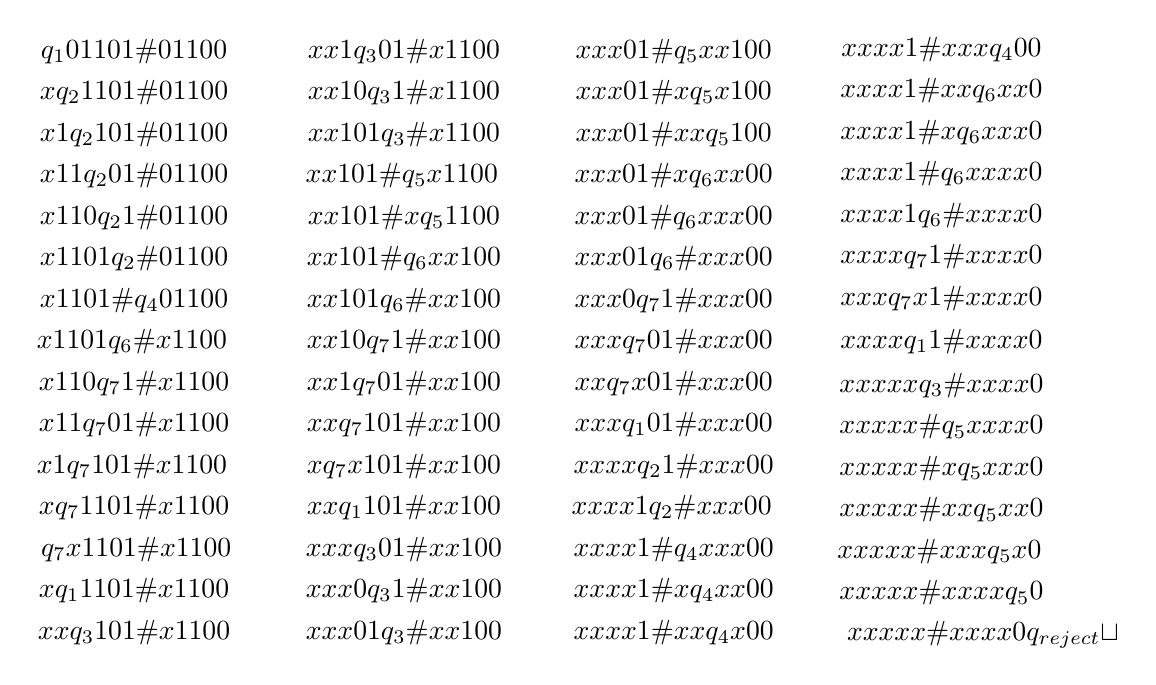
\begin{tikzpicture}[x=0.75pt,y=0.75pt,yscale=-1,xscale=1]
	%uncomment if require: \path (0,359.2857208251953); %set diagram left start at 0, and has height of 359.2857208251953
	
	% Text Node
	\draw (134,35) node  [align=left] {$\displaystyle q_{1} 01101\#01100$};
	% Text Node
	\draw (134,55) node  [align=left] {$\displaystyle xq_{2} 1101\#01100$};
	% Text Node
	\draw (134,75) node  [align=left] {$\displaystyle x1q_{2} 101\#01100$};
	% Text Node
	\draw (134,95) node  [align=left] {$\displaystyle x11q_{2} 01\#01100$};
	% Text Node
	\draw (134,135) node  [align=left] {$\displaystyle x1101q_{2} \#01100$};
	% Text Node
	\draw (134,115) node  [align=left] {$\displaystyle x110q_{2} 1\#01100$};
	% Text Node
	\draw (134,155) node  [align=left] {$\displaystyle x1101 \#q_{4} 01100$};
	% Text Node
	\draw (133,175) node  [align=left] {$\displaystyle x1101q_{6} \#x 1100$};
	% Text Node
	\draw (134,195) node  [align=left] {$\displaystyle x110q_{7} 1\#x 1100$};
	% Text Node
	\draw (134,215) node  [align=left] {$\displaystyle x11q_{7} 01\#x 1100$};
	% Text Node
	\draw (134,255) node  [align=left] {$\displaystyle xq_{7} 1101\#x 1100$};
	% Text Node
	\draw (133,235) node  [align=left] {$\displaystyle x1q_{7} 101\#x 1100$};
	% Text Node
	\draw (135,275) node  [align=left] {$\displaystyle q_{7} x1101\#x 1100$};
	% Text Node
	\draw (134,295) node  [align=left] {$\displaystyle xq_{1} 1101\#x 1100$};
	% Text Node
	\draw (134,315) node  [align=left] {$\displaystyle xxq_{3} 101\#x 1100$};
	% Text Node
	\draw (264,35) node  [align=left] {$\displaystyle xx1q_{3} 01\#x 1100$};
	% Text Node
	\draw (264,75) node  [align=left] {$\displaystyle xx101q_{3} \#x 1100$};
	% Text Node
	\draw (264,55) node  [align=left] {$\displaystyle xx10q_{3} 1\#x 1100$};
	% Text Node
	\draw (263,95) node  [align=left] {$\displaystyle xx101\#q_{5} x 1100$};
	% Text Node
	\draw (264,115) node  [align=left] {$\displaystyle xx101\#xq_{5} 1100$};
	% Text Node
	\draw (264,135) node  [align=left] {$\displaystyle xx101\#q_{6} xx100$};
	% Text Node
	\draw (264,155) node  [align=left] {$\displaystyle xx101q_{6} \#xx100$};
	% Text Node
	\draw (264,175) node  [align=left] {$\displaystyle xx10q_{7} 1\#xx100$};
	% Text Node
	\draw (264,195) node  [align=left] {$\displaystyle xx1q_{7} 01\#xx100$};
	% Text Node
	\draw (264,215) node  [align=left] {$\displaystyle xxq_{7} 101\#xx100$};
	% Text Node
	\draw (264,235) node  [align=left] {$\displaystyle xq_{7} x101\#xx100$};
	% Text Node
	\draw (264,255) node  [align=left] {$\displaystyle xxq_{1} 101\#xx100$};
	% Text Node
	\draw (264,275) node  [align=left] {$\displaystyle xxxq_{3} 01\#xx100$};
	% Text Node
	\draw (264,295) node  [align=left] {$\displaystyle xxx0q_{3} 1\#xx100$};
	% Text Node
	\draw (264,315) node  [align=left] {$\displaystyle xxx01q_{3} \#xx100$};
	% Text Node
	\draw (394,35) node  [align=left] {$\displaystyle xxx01\#q_{5} xx100$};
	% Text Node
	\draw (394,55) node  [align=left] {$\displaystyle xxx01\#xq_{5} x100$};
	% Text Node
	\draw (394,75) node  [align=left] {$\displaystyle xxx01\#xxq_{5} 100$};
	% Text Node
	\draw (394,95) node  [align=left] {$\displaystyle xxx01\#xq_{6} xx00$};
	% Text Node
	\draw (394,115) node  [align=left] {$\displaystyle xxx01\#q_{6} xxx00$};
	% Text Node
	\draw (394,135) node  [align=left] {$\displaystyle xxx01q_{6} \#xxx00$};
	% Text Node
	\draw (394,155) node  [align=left] {$\displaystyle xxx0q_{7} 1\#xxx00$};
	% Text Node
	\draw (394,175) node  [align=left] {$\displaystyle xxxq_{7} 01 \#xxx00$};
	% Text Node
	\draw (394,195) node  [align=left] {$\displaystyle xxq_{7} x 01 \#xxx00$};
	% Text Node
	\draw (394,215) node  [align=left] {$\displaystyle xxxq_{1} 01 \#xxx00$};
	% Text Node
	\draw (394,235) node  [align=left] {$\displaystyle xxxxq_{2} 1\#xxx00$};
	% Text Node
	\draw (393,255) node  [align=left] {$\displaystyle xxxx1q_{2} \#xxx00$};
	% Text Node
	\draw (394,275) node  [align=left] {$\displaystyle xxxx1\#q_{4} xxx00$};
	% Text Node
	\draw (394,295) node  [align=left] {$\displaystyle xxxx1\#xq_{4} xx00$};
	% Text Node
	\draw (394,315) node  [align=left] {$\displaystyle xxxx1\#xxq_{4} x00$};
	% Text Node
	\draw (523,34) node  [align=left] {$\displaystyle xxxx1\#xxxq_{4} 00$};
	% Text Node
	\draw (523,54) node  [align=left] {$\displaystyle xxxx1\#xxq_{6} xx 0$};
	% Text Node
	\draw (523,74) node  [align=left] {$\displaystyle xxxx1\#xq_{6} xxx 0$};
	% Text Node
	\draw (523,114) node  [align=left] {$\displaystyle xxxx1q_{6} \#xxxx 0$};
	% Text Node
	\draw (523,94) node  [align=left] {$\displaystyle xxxx1\#q_{6} xxxx 0$};
	% Text Node
	\draw (523,134) node  [align=left] {$\displaystyle xxxxq_{7} 1\#xxxx 0$};
	% Text Node
	\draw (523,154) node  [align=left] {$\displaystyle xxxq_{7} x1\#xxxx 0$};
	% Text Node
	\draw (523,175) node  [align=left] {$\displaystyle xxxxq_{1} 1\#xxxx 0$};
	% Text Node
	\draw (523,196) node  [align=left] {$\displaystyle xxxxxq_{3} \#xxxx 0$};
	% Text Node
	\draw (523,216) node  [align=left] {$\displaystyle xxxxx\#q_{5} xxxx 0$};
	% Text Node
	\draw (523,236) node  [align=left] {$\displaystyle xxxxx\#xq_{5} xxx 0$};
	% Text Node
	\draw (523,296) node  [align=left] {$\displaystyle xxxxx\#xxxxq_{5} 0$};
	% Text Node
	\draw (523,256) node  [align=left] {$\displaystyle xxxxx\#xxq_{5} xx 0$};
	% Text Node
	\draw (522,276) node  [align=left] {$\displaystyle xxxxx\#xxxq_{5} x 0$};
	% Text Node
	\draw (543,316) node  [align=left] {$\displaystyle xxxxx\#xxxx0q_{reject} \sqcup $};
	
	\end{tikzpicture}

\begin{problem}{3.8}
\end{problem}
\begin{enumerate}
	\item[(b)]
		1. If first alphabet is $\sqcup$, input accepted. 	\\
		2. If first alphabet is 0 write $\sqcup$, move right and jump to step 4. 	\\
		3. If first alphabet is 1 write $\sqcup$, move right and jump to step 8. 	\\

		4. Go right if read x. Repeat till read 0 or 1. 	\\
		5. If read 0, write x, go right till read 1. Write x and go left. 	\\
		6. If read 1, write x, go right till read 0. Write x and go left. 	\\
		7. Go to step 11. 	\\

		8. Go right if read x or 1. Repeat till read 0. 	\\
		9. Write x. Go right if read x or 1. Repeat till read 0. 	\\
		10. Write x and go left. 	\\
		
		11. Go left till read $\sqcup$. Go right. 	\\
		12. Go right if read x. Repeat till read 0, 1 or $\sqcup$. 	\\
		13. If read $\sqcup$, input accepted. 	\\
		14. If read 0, go to step 4. 	\\
		15. If read 1, go to step 8. 	\\

	State diagram: 
	
		\tikzset{every picture/.style={line width=0.75pt}} %set default line width to 0.75pt        
		
		\begin{tikzpicture}[x=0.75pt,y=0.75pt,yscale=-1,xscale=1]
		%uncomment if require: \path (0,564.1428833007812); %set diagram left start at 0, and has height of 564.1428833007812
		
		%Shape: Circle [id:dp5185954568919033] 
		\draw   (323,76) .. controls (323,66.34) and (330.84,58.5) .. (340.5,58.5) .. controls (350.16,58.5) and (358,66.34) .. (358,76) .. controls (358,85.66) and (350.16,93.5) .. (340.5,93.5) .. controls (330.84,93.5) and (323,85.66) .. (323,76) -- cycle ;
		%Shape: Circle [id:dp5295787205846141] 
		\draw   (458,294.5) .. controls (458,284.84) and (465.84,277) .. (475.5,277) .. controls (485.16,277) and (493,284.84) .. (493,294.5) .. controls (493,304.16) and (485.16,312) .. (475.5,312) .. controls (465.84,312) and (458,304.16) .. (458,294.5) -- cycle ;
		%Shape: Circle [id:dp9245890303883415] 
		\draw   (185,295.5) .. controls (185,285.84) and (192.84,278) .. (202.5,278) .. controls (212.16,278) and (220,285.84) .. (220,295.5) .. controls (220,305.16) and (212.16,313) .. (202.5,313) .. controls (192.84,313) and (185,305.16) .. (185,295.5) -- cycle ;
		%Curve Lines [id:da11823075516404935] 
		\draw    (492,287.5) .. controls (535.56,268.69) and (536,320.45) .. (492.34,303.05) ;
		\draw [shift={(491,302.5)}, rotate = 382.89] [color={rgb, 255:red, 0; green, 0; blue, 0 }  ][line width=0.75]    (10.93,-3.29) .. controls (6.95,-1.4) and (3.31,-0.3) .. (0,0) .. controls (3.31,0.3) and (6.95,1.4) .. (10.93,3.29)   ;
		
		%Shape: Circle [id:dp6839429577286817] 
		\draw   (127,373.5) .. controls (127,363.84) and (134.84,356) .. (144.5,356) .. controls (154.16,356) and (162,363.84) .. (162,373.5) .. controls (162,383.16) and (154.16,391) .. (144.5,391) .. controls (134.84,391) and (127,383.16) .. (127,373.5) -- cycle ;
		%Curve Lines [id:da9690224273422121] 
		\draw    (128,366) .. controls (80.48,349.17) and (80,403.89) .. (128.51,383.64) ;
		\draw [shift={(130,383)}, rotate = 516.25] [color={rgb, 255:red, 0; green, 0; blue, 0 }  ][line width=0.75]    (10.93,-3.29) .. controls (6.95,-1.4) and (3.31,-0.3) .. (0,0) .. controls (3.31,0.3) and (6.95,1.4) .. (10.93,3.29)   ;
		
		%Shape: Circle [id:dp9559390115309214] 
		\draw   (322,473.5) .. controls (322,463.84) and (329.84,456) .. (339.5,456) .. controls (349.16,456) and (357,463.84) .. (357,473.5) .. controls (357,483.16) and (349.16,491) .. (339.5,491) .. controls (329.84,491) and (322,483.16) .. (322,473.5) -- cycle ;
		%Shape: Circle [id:dp6804859203364584] 
		\draw   (323,241.5) .. controls (323,231.84) and (330.84,224) .. (340.5,224) .. controls (350.16,224) and (358,231.84) .. (358,241.5) .. controls (358,251.16) and (350.16,259) .. (340.5,259) .. controls (330.84,259) and (323,251.16) .. (323,241.5) -- cycle ;
		%Shape: Circle [id:dp20384745981446661] 
		\draw   (200,374.5) .. controls (200,364.84) and (207.84,357) .. (217.5,357) .. controls (227.16,357) and (235,364.84) .. (235,374.5) .. controls (235,384.16) and (227.16,392) .. (217.5,392) .. controls (207.84,392) and (200,384.16) .. (200,374.5) -- cycle ;
		%Shape: Circle [id:dp8936406964765267] 
		\draw   (323,162) .. controls (323,152.34) and (330.84,144.5) .. (340.5,144.5) .. controls (350.16,144.5) and (358,152.34) .. (358,162) .. controls (358,171.66) and (350.16,179.5) .. (340.5,179.5) .. controls (330.84,179.5) and (323,171.66) .. (323,162) -- cycle ;
		%Straight Lines [id:da6988423327234632] 
		\draw    (353,88.43) -- (465.97,277.71) ;
		\draw [shift={(467,279.43)}, rotate = 239.17000000000002] [color={rgb, 255:red, 0; green, 0; blue, 0 }  ][line width=0.75]    (10.93,-3.29) .. controls (6.95,-1.4) and (3.31,-0.3) .. (0,0) .. controls (3.31,0.3) and (6.95,1.4) .. (10.93,3.29)   ;
		
		%Straight Lines [id:da439481037965445] 
		\draw    (356,248.71) -- (456.14,287.98) ;
		\draw [shift={(458,288.71)}, rotate = 201.41] [color={rgb, 255:red, 0; green, 0; blue, 0 }  ][line width=0.75]    (10.93,-3.29) .. controls (6.95,-1.4) and (3.31,-0.3) .. (0,0) .. controls (3.31,0.3) and (6.95,1.4) .. (10.93,3.29)   ;
		
		%Straight Lines [id:da4430507559977841] 
		\draw    (475.5,312) -- (475.02,355.5) ;
		\draw [shift={(475,357.5)}, rotate = 270.63] [color={rgb, 255:red, 0; green, 0; blue, 0 }  ][line width=0.75]    (10.93,-3.29) .. controls (6.95,-1.4) and (3.31,-0.3) .. (0,0) .. controls (3.31,0.3) and (6.95,1.4) .. (10.93,3.29)   ;
		
		%Shape: Circle [id:dp4870786775429814] 
		\draw   (457.5,375) .. controls (457.5,365.34) and (465.34,357.5) .. (475,357.5) .. controls (484.66,357.5) and (492.5,365.34) .. (492.5,375) .. controls (492.5,384.66) and (484.66,392.5) .. (475,392.5) .. controls (465.34,392.5) and (457.5,384.66) .. (457.5,375) -- cycle ;
		%Curve Lines [id:da7997102445865449] 
		\draw    (491,368.5) .. controls (534.56,349.69) and (535,401.45) .. (491.34,384.05) ;
		\draw [shift={(490,383.5)}, rotate = 382.89] [color={rgb, 255:red, 0; green, 0; blue, 0 }  ][line width=0.75]    (10.93,-3.29) .. controls (6.95,-1.4) and (3.31,-0.3) .. (0,0) .. controls (3.31,0.3) and (6.95,1.4) .. (10.93,3.29)   ;
		
		%Straight Lines [id:da6304229579032048] 
		\draw    (330,89.43) -- (213.05,279.72) ;
		\draw [shift={(212,281.43)}, rotate = 301.57] [color={rgb, 255:red, 0; green, 0; blue, 0 }  ][line width=0.75]    (10.93,-3.29) .. controls (6.95,-1.4) and (3.31,-0.3) .. (0,0) .. controls (3.31,0.3) and (6.95,1.4) .. (10.93,3.29)   ;
		
		%Straight Lines [id:da45269896008275157] 
		\draw    (325,249.71) -- (221.86,289.99) ;
		\draw [shift={(220,290.71)}, rotate = 338.66999999999996] [color={rgb, 255:red, 0; green, 0; blue, 0 }  ][line width=0.75]    (10.93,-3.29) .. controls (6.95,-1.4) and (3.31,-0.3) .. (0,0) .. controls (3.31,0.3) and (6.95,1.4) .. (10.93,3.29)   ;
		
		%Straight Lines [id:da4773256372229189] 
		\draw    (192,309) -- (157.15,358.37) ;
		\draw [shift={(156,360)}, rotate = 305.22] [color={rgb, 255:red, 0; green, 0; blue, 0 }  ][line width=0.75]    (10.93,-3.29) .. controls (6.95,-1.4) and (3.31,-0.3) .. (0,0) .. controls (3.31,0.3) and (6.95,1.4) .. (10.93,3.29)   ;
		
		%Straight Lines [id:da27397385982695965] 
		\draw    (207,312.86) -- (213.21,355.02) ;
		\draw [shift={(213.5,357)}, rotate = 261.62] [color={rgb, 255:red, 0; green, 0; blue, 0 }  ][line width=0.75]    (10.93,-3.29) .. controls (6.95,-1.4) and (3.31,-0.3) .. (0,0) .. controls (3.31,0.3) and (6.95,1.4) .. (10.93,3.29)   ;
		
		%Curve Lines [id:da7789921739554027] 
		\draw    (234,368.5) .. controls (277.56,349.69) and (278,401.45) .. (234.34,384.05) ;
		\draw [shift={(233,383.5)}, rotate = 382.89] [color={rgb, 255:red, 0; green, 0; blue, 0 }  ][line width=0.75]    (10.93,-3.29) .. controls (6.95,-1.4) and (3.31,-0.3) .. (0,0) .. controls (3.31,0.3) and (6.95,1.4) .. (10.93,3.29)   ;
		
		%Straight Lines [id:da49186849437766966] 
		\draw    (229,387.86) -- (324.4,459.8) ;
		\draw [shift={(326,461)}, rotate = 217.02] [color={rgb, 255:red, 0; green, 0; blue, 0 }  ][line width=0.75]    (10.93,-3.29) .. controls (6.95,-1.4) and (3.31,-0.3) .. (0,0) .. controls (3.31,0.3) and (6.95,1.4) .. (10.93,3.29)   ;
		
		%Straight Lines [id:da07357319086983694] 
		\draw    (155,387) -- (321.19,466.14) ;
		\draw [shift={(323,467)}, rotate = 205.46] [color={rgb, 255:red, 0; green, 0; blue, 0 }  ][line width=0.75]    (10.93,-3.29) .. controls (6.95,-1.4) and (3.31,-0.3) .. (0,0) .. controls (3.31,0.3) and (6.95,1.4) .. (10.93,3.29)   ;
		
		%Straight Lines [id:da640085315743254] 
		\draw    (462,386) -- (354.63,462.84) ;
		\draw [shift={(353,464)}, rotate = 324.40999999999997] [color={rgb, 255:red, 0; green, 0; blue, 0 }  ][line width=0.75]    (10.93,-3.29) .. controls (6.95,-1.4) and (3.31,-0.3) .. (0,0) .. controls (3.31,0.3) and (6.95,1.4) .. (10.93,3.29)   ;
		
		%Curve Lines [id:da40752850163427334] 
		\draw    (330,489) .. controls (300.3,541.47) and (381.35,544.94) .. (350.96,488.72) ;
		\draw [shift={(350,487)}, rotate = 420.36] [color={rgb, 255:red, 0; green, 0; blue, 0 }  ][line width=0.75]    (10.93,-3.29) .. controls (6.95,-1.4) and (3.31,-0.3) .. (0,0) .. controls (3.31,0.3) and (6.95,1.4) .. (10.93,3.29)   ;
		
		%Curve Lines [id:da7873721132604454] 
		\draw    (331,227.71) .. controls (304.4,202.1) and (281.69,238.59) .. (321.15,241.4) ;
		\draw [shift={(323,241.5)}, rotate = 182.43] [color={rgb, 255:red, 0; green, 0; blue, 0 }  ][line width=0.75]    (10.93,-3.29) .. controls (6.95,-1.4) and (3.31,-0.3) .. (0,0) .. controls (3.31,0.3) and (6.95,1.4) .. (10.93,3.29)   ;
		
		%Straight Lines [id:da21193570993598798] 
		\draw    (340.5,224) -- (340.5,181.5) ;
		\draw [shift={(340.5,179.5)}, rotate = 450] [color={rgb, 255:red, 0; green, 0; blue, 0 }  ][line width=0.75]    (10.93,-3.29) .. controls (6.95,-1.4) and (3.31,-0.3) .. (0,0) .. controls (3.31,0.3) and (6.95,1.4) .. (10.93,3.29)   ;
		
		%Straight Lines [id:da13263402792723467] 
		\draw    (340,18.5) -- (340.48,56.5) ;
		\draw [shift={(340.5,58.5)}, rotate = 269.28] [color={rgb, 255:red, 0; green, 0; blue, 0 }  ][line width=0.75]    (10.93,-3.29) .. controls (6.95,-1.4) and (3.31,-0.3) .. (0,0) .. controls (3.31,0.3) and (6.95,1.4) .. (10.93,3.29)   ;
		
		%Straight Lines [id:da7660045417395827] 
		\draw    (340.5,93.5) -- (340.5,142.5) ;
		\draw [shift={(340.5,144.5)}, rotate = 270] [color={rgb, 255:red, 0; green, 0; blue, 0 }  ][line width=0.75]    (10.93,-3.29) .. controls (6.95,-1.4) and (3.31,-0.3) .. (0,0) .. controls (3.31,0.3) and (6.95,1.4) .. (10.93,3.29)   ;
		
		%Curve Lines [id:da2148608951501918] 
		\draw    (186,289) .. controls (138.48,272.17) and (138,326.89) .. (186.51,306.64) ;
		\draw [shift={(188,306)}, rotate = 516.25] [color={rgb, 255:red, 0; green, 0; blue, 0 }  ][line width=0.75]    (10.93,-3.29) .. controls (6.95,-1.4) and (3.31,-0.3) .. (0,0) .. controls (3.31,0.3) and (6.95,1.4) .. (10.93,3.29)   ;
		
		%Straight Lines [id:da5632720397453483] 
		\draw    (339.5,456) -- (340.49,261) ;
		\draw [shift={(340.5,259)}, rotate = 450.29] [color={rgb, 255:red, 0; green, 0; blue, 0 }  ][line width=0.75]    (10.93,-3.29) .. controls (6.95,-1.4) and (3.31,-0.3) .. (0,0) .. controls (3.31,0.3) and (6.95,1.4) .. (10.93,3.29)   ;
		
		% Text Node
		\draw (278,92) node  [align=left] {$\displaystyle 0\shortrightarrow \sqcup ,R$};
		% Text Node
		\draw (420,91) node  [align=left] {$\displaystyle 1\shortrightarrow \sqcup ,R$};
		% Text Node
		\draw (518,333) node  [align=left] {$\displaystyle 0\shortrightarrow x,R$};
		% Text Node
		\draw (471,409) node  [align=left] {$\displaystyle 0\shortrightarrow x,L$};
		% Text Node
		\draw (143,327) node  [align=left] {$\displaystyle 0\shortrightarrow x,R$};
		% Text Node
		\draw (164,410) node  [align=left] {$\displaystyle 1\shortrightarrow x,L$};
		% Text Node
		\draw (345,544) node  [align=left] {$\displaystyle 0,1,x\shortrightarrow L$};
		% Text Node
		\draw (226,323) node  [align=left] {$\displaystyle 1\shortrightarrow x,R$};
		% Text Node
		\draw (256,402) node  [align=left] {$\displaystyle 0\shortrightarrow x,L$};
		% Text Node
		\draw (290,230) node  [align=left] {$\displaystyle x\shortrightarrow R$};
		% Text Node
		\draw (339,207) node  [align=left] {$\displaystyle \sqcup \shortrightarrow R$};
		% Text Node
		\draw (286,266) node  [align=left] {$\displaystyle 0\shortrightarrow x,R$};
		% Text Node
		\draw (407,268.71) node  [align=left] {$\displaystyle 1\shortrightarrow x,R$};
		% Text Node
		\draw (340.5,119) node  [align=left] {$\displaystyle \sqcup \shortrightarrow R$};
		% Text Node
		\draw (338,427) node  [align=left] {$\displaystyle \sqcup \shortrightarrow R$};
		% Text Node
		\draw (340.5,76) node  [align=left] {$\displaystyle q_{1}$};
		% Text Node
		\draw (202.5,295.5) node  [align=left] {$\displaystyle q_{2}$};
		% Text Node
		\draw (475.5,294.5) node  [align=left] {$\displaystyle q_{3}$};
		% Text Node
		\draw (144.5,373.5) node  [align=left] {$\displaystyle q_{4}$};
		% Text Node
		\draw (217.5,374.5) node  [align=left] {$\displaystyle q_{5}$};
		% Text Node
		\draw (475,375) node  [align=left] {$\displaystyle q_{6}$};
		% Text Node
		\draw (339.5,473.5) node  [align=left] {$\displaystyle q_{7}$};
		% Text Node
		\draw (340.5,241.5) node  [align=left] {$\displaystyle q_{8}$};
		% Text Node
		\draw (340.5,162) node  [align=left] {$\displaystyle q_{accept}$};
		% Text Node
		\draw (125,299) node  [align=left] {$\displaystyle x\shortrightarrow R$};
		% Text Node
		\draw (60,375) node  [align=left] {$\displaystyle 0,x\shortrightarrow R$};
		% Text Node
		\draw (302,376) node  [align=left] {$\displaystyle 1,x\shortrightarrow R$};
		% Text Node
		\draw (559,293) node  [align=left] {$\displaystyle 1,x\shortrightarrow R$};
		% Text Node
		\draw (559,376) node  [align=left] {$\displaystyle 1,x\shortrightarrow R$};
		
		\end{tikzpicture}
	
	Input string 010100: 
	
		\tikzset{every picture/.style={line width=0.75pt}} %set default line width to 0.75pt        
		
		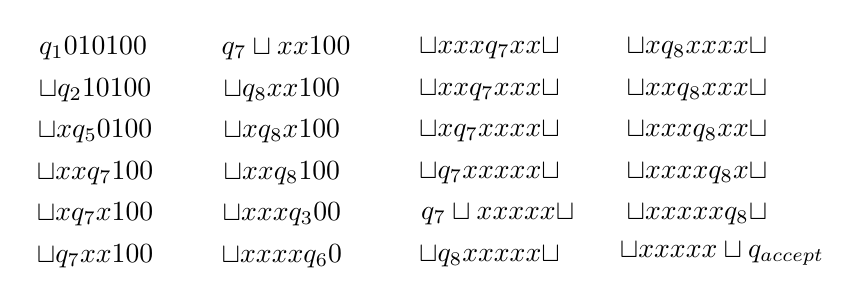
\begin{tikzpicture}[x=0.75pt,y=0.75pt,yscale=-1,xscale=1]
		%uncomment if require: \path (0,327.2857131958008); %set diagram left start at 0, and has height of 327.2857131958008
		
		% Text Node
		\draw (133,45) node  [align=left] {$\displaystyle q_{1} 010100$};
		% Text Node
		\draw (134,65) node  [align=left] {$\displaystyle \sqcup q_{2} 10100$};
		% Text Node
		\draw (134,85) node  [align=left] {$\displaystyle \sqcup xq_{5} 0100$};
		% Text Node
		\draw (134,105) node  [align=left] {$\displaystyle \sqcup xxq_{7} 100$};
		% Text Node
		\draw (134,125) node  [align=left] {$\displaystyle \sqcup xq_{7} x100$};
		% Text Node
		\draw (226,45) node  [align=left] {$\displaystyle q_{7} \sqcup xx 100$};
		% Text Node
		\draw (134,145) node  [align=left] {$\displaystyle \sqcup q_{7} xx100$};
		% Text Node
		\draw (224,65) node  [align=left] {$\displaystyle \sqcup q_{8} xx 100$};
		% Text Node
		\draw (224,85) node  [align=left] {$\displaystyle \sqcup xq_{8} x 100$};
		% Text Node
		\draw (224,105) node  [align=left] {$\displaystyle \sqcup xxq_{8} 100$};
		% Text Node
		\draw (224,125) node  [align=left] {$\displaystyle \sqcup xxxq_{3} 00$};
		% Text Node
		\draw (224,145) node  [align=left] {$\displaystyle \sqcup xxxxq_{6} 0$};
		% Text Node
		\draw (324,65) node  [align=left] {$\displaystyle \sqcup xxq_{7} xxx\sqcup $};
		% Text Node
		\draw (324,45) node  [align=left] {$\displaystyle \sqcup xxxq_{7} xx\sqcup $};
		% Text Node
		\draw (324,105) node  [align=left] {$\displaystyle \sqcup q_{7} xxxxx\sqcup $};
		% Text Node
		\draw (328,125) node  [align=left] {$\displaystyle q_{7} \sqcup xxxxx\sqcup $};
		% Text Node
		\draw (324,85) node  [align=left] {$\displaystyle \sqcup xq_{7} xxxx\sqcup $};
		% Text Node
		\draw (324,145) node  [align=left] {$\displaystyle \sqcup q_{8} xxxxx\sqcup $};
		% Text Node
		\draw (424,45) node  [align=left] {$\displaystyle \sqcup xq_{8} xxxx\sqcup $};
		% Text Node
		\draw (424,125) node  [align=left] {$\displaystyle \sqcup xxxxxq_{8} \sqcup $};
		% Text Node
		\draw (424,105) node  [align=left] {$\displaystyle \sqcup xxxxq_{8} x\sqcup $};
		% Text Node
		\draw (424,85) node  [align=left] {$\displaystyle \sqcup xxxq_{8} xx\sqcup $};
		% Text Node
		\draw (424,65) node  [align=left] {$\displaystyle \sqcup xxq_{8} xxx\sqcup $};
		% Text Node
		\draw (436,144) node  [align=left] {$\displaystyle \sqcup xxxxx\sqcup q_{accept}$};
		
		\end{tikzpicture}
	
	Input string 010101: 
	
		\tikzset{every picture/.style={line width=0.75pt}} %set default line width to 0.75pt        
		
		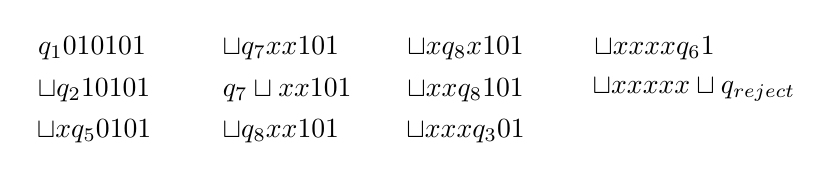
\begin{tikzpicture}[x=0.75pt,y=0.75pt,yscale=-1,xscale=1]
		%uncomment if require: \path (0,216.5); %set diagram left start at 0, and has height of 216.5
		
		% Text Node
		\draw (133,45) node  [align=left] {$\displaystyle q_{1} 010101$};
		% Text Node
		\draw (134,65) node  [align=left] {$\displaystyle \sqcup q_{2} 10101$};
		% Text Node
		\draw (134,85) node  [align=left] {$\displaystyle \sqcup xq_{5} 0101$};
		% Text Node
		\draw (227,65) node  [align=left] {$\displaystyle q_{7} \sqcup xx 101$};
		% Text Node
		\draw (224,45) node  [align=left] {$\displaystyle \sqcup q_{7} xx101$};
		% Text Node
		\draw (224,85) node  [align=left] {$\displaystyle \sqcup q_{8} xx 101$};
		% Text Node
		\draw (313,45) node  [align=left] {$\displaystyle \sqcup xq_{8} x 101$};
		% Text Node
		\draw (313,65) node  [align=left] {$\displaystyle \sqcup xxq_{8} 101$};
		% Text Node
		\draw (313,85) node  [align=left] {$\displaystyle \sqcup xxxq_{3} 01$};
		% Text Node
		\draw (404,45) node  [align=left] {$\displaystyle \sqcup xxxxq_{6} 1$};
		% Text Node
		\draw (423,65) node  [align=left] {$\displaystyle \sqcup xxxxx\sqcup q_{reject}$};
		
		\end{tikzpicture}

	\item[(c)]
		1. If first alphabet is $\sqcup$, input rejected. 	\\
		2. If first alphabet is 0 write $\sqcup$, move right and jump to step 4. 	\\
		3. If first alphabet is 1 write $\sqcup$, move right and jump to step 8. 	\\

		4. Go right if read x. Repeat till read 0 or 1. 	\\
		5. If read 0, write x, go right till read 1. Write x and go left. 	\\
		6. If read 1, write x, go right till read 0. Write x and go left. 	\\
		7. Go to step 11. 	\\

		8. Go right if read x or 1. Repeat till read 0. 	\\
		9. Write x. Go right if read x or 1. Repeat till read 0. 	\\
		10. Write x and go left. 	\\
		
		11. Go left till read $\sqcup$. Go right. 	\\
		12. Go right if read x. Repeat till read 0, 1 or $\sqcup$. 	\\
		13. If read $\sqcup$, input rejected. 	\\
		14. If read 0, go to step 4. 	\\
		15. If read 1, go to step 8. 	\\

		State diagram: 
		
			\tikzset{every picture/.style={line width=0.75pt}} %set default line width to 0.75pt        
			
			\begin{tikzpicture}[x=0.75pt,y=0.75pt,yscale=-1,xscale=1]
			%uncomment if require: \path (0,564.1428833007812); %set diagram left start at 0, and has height of 564.1428833007812
			
			%Shape: Circle [id:dp9858799087828809] 
			\draw   (323,76) .. controls (323,66.34) and (330.84,58.5) .. (340.5,58.5) .. controls (350.16,58.5) and (358,66.34) .. (358,76) .. controls (358,85.66) and (350.16,93.5) .. (340.5,93.5) .. controls (330.84,93.5) and (323,85.66) .. (323,76) -- cycle ;
			%Shape: Circle [id:dp055810369076301436] 
			\draw   (458,294.5) .. controls (458,284.84) and (465.84,277) .. (475.5,277) .. controls (485.16,277) and (493,284.84) .. (493,294.5) .. controls (493,304.16) and (485.16,312) .. (475.5,312) .. controls (465.84,312) and (458,304.16) .. (458,294.5) -- cycle ;
			%Shape: Circle [id:dp9513697631913915] 
			\draw   (185,295.5) .. controls (185,285.84) and (192.84,278) .. (202.5,278) .. controls (212.16,278) and (220,285.84) .. (220,295.5) .. controls (220,305.16) and (212.16,313) .. (202.5,313) .. controls (192.84,313) and (185,305.16) .. (185,295.5) -- cycle ;
			%Curve Lines [id:da8210262283316048] 
			\draw    (492,287.5) .. controls (535.56,268.69) and (536,320.45) .. (492.34,303.05) ;
			\draw [shift={(491,302.5)}, rotate = 382.89] [color={rgb, 255:red, 0; green, 0; blue, 0 }  ][line width=0.75]    (10.93,-3.29) .. controls (6.95,-1.4) and (3.31,-0.3) .. (0,0) .. controls (3.31,0.3) and (6.95,1.4) .. (10.93,3.29)   ;
			
			%Shape: Circle [id:dp8930202448952342] 
			\draw   (127,373.5) .. controls (127,363.84) and (134.84,356) .. (144.5,356) .. controls (154.16,356) and (162,363.84) .. (162,373.5) .. controls (162,383.16) and (154.16,391) .. (144.5,391) .. controls (134.84,391) and (127,383.16) .. (127,373.5) -- cycle ;
			%Curve Lines [id:da816548813009742] 
			\draw    (128,366) .. controls (80.48,349.17) and (80,403.89) .. (128.51,383.64) ;
			\draw [shift={(130,383)}, rotate = 516.25] [color={rgb, 255:red, 0; green, 0; blue, 0 }  ][line width=0.75]    (10.93,-3.29) .. controls (6.95,-1.4) and (3.31,-0.3) .. (0,0) .. controls (3.31,0.3) and (6.95,1.4) .. (10.93,3.29)   ;
			
			%Shape: Circle [id:dp257985409172536] 
			\draw   (322,473.5) .. controls (322,463.84) and (329.84,456) .. (339.5,456) .. controls (349.16,456) and (357,463.84) .. (357,473.5) .. controls (357,483.16) and (349.16,491) .. (339.5,491) .. controls (329.84,491) and (322,483.16) .. (322,473.5) -- cycle ;
			%Shape: Circle [id:dp1862964316739364] 
			\draw   (323,241.5) .. controls (323,231.84) and (330.84,224) .. (340.5,224) .. controls (350.16,224) and (358,231.84) .. (358,241.5) .. controls (358,251.16) and (350.16,259) .. (340.5,259) .. controls (330.84,259) and (323,251.16) .. (323,241.5) -- cycle ;
			%Shape: Circle [id:dp8956791800178956] 
			\draw   (200,374.5) .. controls (200,364.84) and (207.84,357) .. (217.5,357) .. controls (227.16,357) and (235,364.84) .. (235,374.5) .. controls (235,384.16) and (227.16,392) .. (217.5,392) .. controls (207.84,392) and (200,384.16) .. (200,374.5) -- cycle ;
			%Shape: Circle [id:dp7485389063849635] 
			\draw   (323,162) .. controls (323,152.34) and (330.84,144.5) .. (340.5,144.5) .. controls (350.16,144.5) and (358,152.34) .. (358,162) .. controls (358,171.66) and (350.16,179.5) .. (340.5,179.5) .. controls (330.84,179.5) and (323,171.66) .. (323,162) -- cycle ;
			%Straight Lines [id:da039127268332023846] 
			\draw    (353,88.43) -- (465.97,277.71) ;
			\draw [shift={(467,279.43)}, rotate = 239.17000000000002] [color={rgb, 255:red, 0; green, 0; blue, 0 }  ][line width=0.75]    (10.93,-3.29) .. controls (6.95,-1.4) and (3.31,-0.3) .. (0,0) .. controls (3.31,0.3) and (6.95,1.4) .. (10.93,3.29)   ;
			
			%Straight Lines [id:da538384584927889] 
			\draw    (356,248.71) -- (456.14,287.98) ;
			\draw [shift={(458,288.71)}, rotate = 201.41] [color={rgb, 255:red, 0; green, 0; blue, 0 }  ][line width=0.75]    (10.93,-3.29) .. controls (6.95,-1.4) and (3.31,-0.3) .. (0,0) .. controls (3.31,0.3) and (6.95,1.4) .. (10.93,3.29)   ;
			
			%Straight Lines [id:da29523119715242174] 
			\draw    (475.5,312) -- (475.02,355.5) ;
			\draw [shift={(475,357.5)}, rotate = 270.63] [color={rgb, 255:red, 0; green, 0; blue, 0 }  ][line width=0.75]    (10.93,-3.29) .. controls (6.95,-1.4) and (3.31,-0.3) .. (0,0) .. controls (3.31,0.3) and (6.95,1.4) .. (10.93,3.29)   ;
			
			%Shape: Circle [id:dp9247727612862384] 
			\draw   (457.5,375) .. controls (457.5,365.34) and (465.34,357.5) .. (475,357.5) .. controls (484.66,357.5) and (492.5,365.34) .. (492.5,375) .. controls (492.5,384.66) and (484.66,392.5) .. (475,392.5) .. controls (465.34,392.5) and (457.5,384.66) .. (457.5,375) -- cycle ;
			%Curve Lines [id:da2718647581952185] 
			\draw    (491,368.5) .. controls (534.56,349.69) and (535,401.45) .. (491.34,384.05) ;
			\draw [shift={(490,383.5)}, rotate = 382.89] [color={rgb, 255:red, 0; green, 0; blue, 0 }  ][line width=0.75]    (10.93,-3.29) .. controls (6.95,-1.4) and (3.31,-0.3) .. (0,0) .. controls (3.31,0.3) and (6.95,1.4) .. (10.93,3.29)   ;
			
			%Straight Lines [id:da00944562782813052] 
			\draw    (330,89.43) -- (213.05,279.72) ;
			\draw [shift={(212,281.43)}, rotate = 301.57] [color={rgb, 255:red, 0; green, 0; blue, 0 }  ][line width=0.75]    (10.93,-3.29) .. controls (6.95,-1.4) and (3.31,-0.3) .. (0,0) .. controls (3.31,0.3) and (6.95,1.4) .. (10.93,3.29)   ;
			
			%Straight Lines [id:da13585226480244916] 
			\draw    (325,249.71) -- (221.86,289.99) ;
			\draw [shift={(220,290.71)}, rotate = 338.66999999999996] [color={rgb, 255:red, 0; green, 0; blue, 0 }  ][line width=0.75]    (10.93,-3.29) .. controls (6.95,-1.4) and (3.31,-0.3) .. (0,0) .. controls (3.31,0.3) and (6.95,1.4) .. (10.93,3.29)   ;
			
			%Straight Lines [id:da06728544160023109] 
			\draw    (192,309) -- (157.15,358.37) ;
			\draw [shift={(156,360)}, rotate = 305.22] [color={rgb, 255:red, 0; green, 0; blue, 0 }  ][line width=0.75]    (10.93,-3.29) .. controls (6.95,-1.4) and (3.31,-0.3) .. (0,0) .. controls (3.31,0.3) and (6.95,1.4) .. (10.93,3.29)   ;
			
			%Straight Lines [id:da21345269929298172] 
			\draw    (207,312.86) -- (213.21,355.02) ;
			\draw [shift={(213.5,357)}, rotate = 261.62] [color={rgb, 255:red, 0; green, 0; blue, 0 }  ][line width=0.75]    (10.93,-3.29) .. controls (6.95,-1.4) and (3.31,-0.3) .. (0,0) .. controls (3.31,0.3) and (6.95,1.4) .. (10.93,3.29)   ;
			
			%Curve Lines [id:da7416755679353784] 
			\draw    (234,368.5) .. controls (277.56,349.69) and (278,401.45) .. (234.34,384.05) ;
			\draw [shift={(233,383.5)}, rotate = 382.89] [color={rgb, 255:red, 0; green, 0; blue, 0 }  ][line width=0.75]    (10.93,-3.29) .. controls (6.95,-1.4) and (3.31,-0.3) .. (0,0) .. controls (3.31,0.3) and (6.95,1.4) .. (10.93,3.29)   ;
			
			%Straight Lines [id:da5468183758324205] 
			\draw    (229,387.86) -- (324.4,459.8) ;
			\draw [shift={(326,461)}, rotate = 217.02] [color={rgb, 255:red, 0; green, 0; blue, 0 }  ][line width=0.75]    (10.93,-3.29) .. controls (6.95,-1.4) and (3.31,-0.3) .. (0,0) .. controls (3.31,0.3) and (6.95,1.4) .. (10.93,3.29)   ;
			
			%Straight Lines [id:da2507386757393626] 
			\draw    (155,387) -- (321.19,466.14) ;
			\draw [shift={(323,467)}, rotate = 205.46] [color={rgb, 255:red, 0; green, 0; blue, 0 }  ][line width=0.75]    (10.93,-3.29) .. controls (6.95,-1.4) and (3.31,-0.3) .. (0,0) .. controls (3.31,0.3) and (6.95,1.4) .. (10.93,3.29)   ;
			
			%Straight Lines [id:da5468013585621889] 
			\draw    (462,386) -- (354.63,462.84) ;
			\draw [shift={(353,464)}, rotate = 324.40999999999997] [color={rgb, 255:red, 0; green, 0; blue, 0 }  ][line width=0.75]    (10.93,-3.29) .. controls (6.95,-1.4) and (3.31,-0.3) .. (0,0) .. controls (3.31,0.3) and (6.95,1.4) .. (10.93,3.29)   ;
			
			%Curve Lines [id:da04005143118398391] 
			\draw    (330,489) .. controls (300.3,541.47) and (381.35,544.94) .. (350.96,488.72) ;
			\draw [shift={(350,487)}, rotate = 420.36] [color={rgb, 255:red, 0; green, 0; blue, 0 }  ][line width=0.75]    (10.93,-3.29) .. controls (6.95,-1.4) and (3.31,-0.3) .. (0,0) .. controls (3.31,0.3) and (6.95,1.4) .. (10.93,3.29)   ;
			
			%Curve Lines [id:da7856717447765169] 
			\draw    (331,227.71) .. controls (304.4,202.1) and (281.69,238.59) .. (321.15,241.4) ;
			\draw [shift={(323,241.5)}, rotate = 182.43] [color={rgb, 255:red, 0; green, 0; blue, 0 }  ][line width=0.75]    (10.93,-3.29) .. controls (6.95,-1.4) and (3.31,-0.3) .. (0,0) .. controls (3.31,0.3) and (6.95,1.4) .. (10.93,3.29)   ;
			
			%Straight Lines [id:da6700438749514337] 
			\draw    (340.5,224) -- (340.5,181.5) ;
			\draw [shift={(340.5,179.5)}, rotate = 450] [color={rgb, 255:red, 0; green, 0; blue, 0 }  ][line width=0.75]    (10.93,-3.29) .. controls (6.95,-1.4) and (3.31,-0.3) .. (0,0) .. controls (3.31,0.3) and (6.95,1.4) .. (10.93,3.29)   ;
			
			%Straight Lines [id:da7120822467495782] 
			\draw    (340,18.5) -- (340.48,56.5) ;
			\draw [shift={(340.5,58.5)}, rotate = 269.28] [color={rgb, 255:red, 0; green, 0; blue, 0 }  ][line width=0.75]    (10.93,-3.29) .. controls (6.95,-1.4) and (3.31,-0.3) .. (0,0) .. controls (3.31,0.3) and (6.95,1.4) .. (10.93,3.29)   ;
			
			%Straight Lines [id:da53761501071465] 
			\draw    (340.5,93.5) -- (340.5,142.5) ;
			\draw [shift={(340.5,144.5)}, rotate = 270] [color={rgb, 255:red, 0; green, 0; blue, 0 }  ][line width=0.75]    (10.93,-3.29) .. controls (6.95,-1.4) and (3.31,-0.3) .. (0,0) .. controls (3.31,0.3) and (6.95,1.4) .. (10.93,3.29)   ;
			
			%Curve Lines [id:da42588595437136645] 
			\draw    (186,289) .. controls (138.48,272.17) and (138,326.89) .. (186.51,306.64) ;
			\draw [shift={(188,306)}, rotate = 516.25] [color={rgb, 255:red, 0; green, 0; blue, 0 }  ][line width=0.75]    (10.93,-3.29) .. controls (6.95,-1.4) and (3.31,-0.3) .. (0,0) .. controls (3.31,0.3) and (6.95,1.4) .. (10.93,3.29)   ;
			
			%Straight Lines [id:da7845890729174243] 
			\draw    (339.5,456) -- (340.49,261) ;
			\draw [shift={(340.5,259)}, rotate = 450.29] [color={rgb, 255:red, 0; green, 0; blue, 0 }  ][line width=0.75]    (10.93,-3.29) .. controls (6.95,-1.4) and (3.31,-0.3) .. (0,0) .. controls (3.31,0.3) and (6.95,1.4) .. (10.93,3.29)   ;
			
			% Text Node
			\draw (278,92) node  [align=left] {$\displaystyle 0\shortrightarrow \sqcup ,R$};
			% Text Node
			\draw (420,91) node  [align=left] {$\displaystyle 1\shortrightarrow \sqcup ,R$};
			% Text Node
			\draw (518,333) node  [align=left] {$\displaystyle 0\shortrightarrow x,R$};
			% Text Node
			\draw (471,409) node  [align=left] {$\displaystyle 0\shortrightarrow x,L$};
			% Text Node
			\draw (143,327) node  [align=left] {$\displaystyle 0\shortrightarrow x,R$};
			% Text Node
			\draw (164,410) node  [align=left] {$\displaystyle 1\shortrightarrow x,L$};
			% Text Node
			\draw (345,544) node  [align=left] {$\displaystyle 0,1,x\shortrightarrow L$};
			% Text Node
			\draw (226,323) node  [align=left] {$\displaystyle 1\shortrightarrow x,R$};
			% Text Node
			\draw (256,402) node  [align=left] {$\displaystyle 0\shortrightarrow x,L$};
			% Text Node
			\draw (290,230) node  [align=left] {$\displaystyle x\shortrightarrow R$};
			% Text Node
			\draw (339,207) node  [align=left] {$\displaystyle \sqcup \shortrightarrow R$};
			% Text Node
			\draw (286,266) node  [align=left] {$\displaystyle 0\shortrightarrow x,R$};
			% Text Node
			\draw (407,268.71) node  [align=left] {$\displaystyle 1\shortrightarrow x,R$};
			% Text Node
			\draw (340.5,119) node  [align=left] {$\displaystyle \sqcup \shortrightarrow R$};
			% Text Node
			\draw (338,427) node  [align=left] {$\displaystyle \sqcup \shortrightarrow R$};
			% Text Node
			\draw (340.5,76) node  [align=left] {$\displaystyle q_{1}$};
			% Text Node
			\draw (202.5,295.5) node  [align=left] {$\displaystyle q_{2}$};
			% Text Node
			\draw (475.5,294.5) node  [align=left] {$\displaystyle q_{3}$};
			% Text Node
			\draw (144.5,373.5) node  [align=left] {$\displaystyle q_{4}$};
			% Text Node
			\draw (217.5,374.5) node  [align=left] {$\displaystyle q_{5}$};
			% Text Node
			\draw (475,375) node  [align=left] {$\displaystyle q_{6}$};
			% Text Node
			\draw (339.5,473.5) node  [align=left] {$\displaystyle q_{7}$};
			% Text Node
			\draw (340.5,241.5) node  [align=left] {$\displaystyle q_{8}$};
			% Text Node
			\draw (340.5,162) node  [align=left] {$\displaystyle q_{reject}$};
			% Text Node
			\draw (125,299) node  [align=left] {$\displaystyle x\shortrightarrow R$};
			% Text Node
			\draw (60,375) node  [align=left] {$\displaystyle 0,x\shortrightarrow R$};
			% Text Node
			\draw (302,376) node  [align=left] {$\displaystyle 1,x\shortrightarrow R$};
			% Text Node
			\draw (559,293) node  [align=left] {$\displaystyle 1,x\shortrightarrow R$};
			% Text Node
			\draw (559,376) node  [align=left] {$\displaystyle 1,x\shortrightarrow R$};
			
			\end{tikzpicture}
		
		Input string 000111: 
		
			\tikzset{every picture/.style={line width=0.75pt}} %set default line width to 0.75pt        
			
			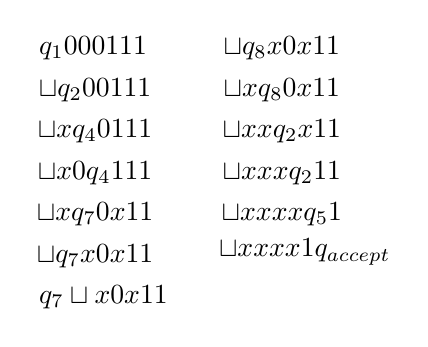
\begin{tikzpicture}[x=0.75pt,y=0.75pt,yscale=-1,xscale=1]
			%uncomment if require: \path (0,243); %set diagram left start at 0, and has height of 243
			
			% Text Node
			\draw (268,36) node  [align=left] {$ $};
			% Text Node
			\draw (262,25) node  [align=left] {$\displaystyle q_{1} 000111$};
			% Text Node
			\draw (263,45) node  [align=left] {$\displaystyle \sqcup q_{2} 00111$};
			% Text Node
			\draw (263,65) node  [align=left] {$\displaystyle \sqcup xq_{4} 0111$};
			% Text Node
			\draw (263,85) node  [align=left] {$\displaystyle \sqcup x0q_{4} 111$};
			% Text Node
			\draw (263,105) node  [align=left] {$\displaystyle \sqcup xq_{7} 0x11$};
			% Text Node
			\draw (267,145) node  [align=left] {$\displaystyle q_{7} \sqcup x0x11$};
			% Text Node
			\draw (263,125) node  [align=left] {$\displaystyle \sqcup q_{7} x0x11$};
			% Text Node
			\draw (353,25) node  [align=left] {$\displaystyle \sqcup q_{8} x0x11$};
			% Text Node
			\draw (353,45) node  [align=left] {$\displaystyle \sqcup xq_{8} 0x11$};
			% Text Node
			\draw (353,65) node  [align=left] {$\displaystyle \sqcup xxq_{2} x11$};
			% Text Node
			\draw (353,85) node  [align=left] {$\displaystyle \sqcup xxxq_{2} 11$};
			% Text Node
			\draw (353,105) node  [align=left] {$\displaystyle \sqcup xxxxq_{5} 1$};
			% Text Node
			\draw (364,123) node  [align=left] {$\displaystyle \sqcup xxxx 1q_{accept}$};
			
			\end{tikzpicture}
		
		Input string 000110: 
		
			\tikzset{every picture/.style={line width=0.75pt}} %set default line width to 0.75pt        
			
			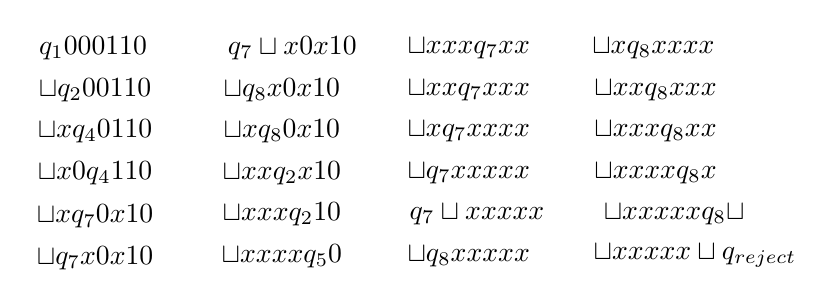
\begin{tikzpicture}[x=0.75pt,y=0.75pt,yscale=-1,xscale=1]
			%uncomment if require: \path (0,296.5); %set diagram left start at 0, and has height of 296.5
			
			% Text Node
			\draw (159,66) node  [align=left] {$ $};
			% Text Node
			\draw (153,55) node  [align=left] {$\displaystyle q_{1} 000110$};
			% Text Node
			\draw (154,75) node  [align=left] {$\displaystyle \sqcup q_{2} 00110$};
			% Text Node
			\draw (154,95) node  [align=left] {$\displaystyle \sqcup xq_{4} 0110$};
			% Text Node
			\draw (154,115) node  [align=left] {$\displaystyle \sqcup x0q_{4} 110$};
			% Text Node
			\draw (154,136) node  [align=left] {$\displaystyle \sqcup xq_{7} 0x10$};
			% Text Node
			\draw (249,55) node  [align=left] {$\displaystyle q_{7} \sqcup x0x10$};
			% Text Node
			\draw (154,156) node  [align=left] {$\displaystyle \sqcup q_{7} x0x10$};
			% Text Node
			\draw (244,75) node  [align=left] {$\displaystyle \sqcup q_{8} x0x10$};
			% Text Node
			\draw (244,95) node  [align=left] {$\displaystyle \sqcup xq_{8} 0x10$};
			% Text Node
			\draw (244,115) node  [align=left] {$\displaystyle \sqcup xxq_{2} x10$};
			% Text Node
			\draw (244,135) node  [align=left] {$\displaystyle \sqcup xxxq_{2} 10$};
			% Text Node
			\draw (244,155) node  [align=left] {$\displaystyle \sqcup xxxxq_{5} 0$};
			% Text Node
			\draw (334,55) node  [align=left] {$\displaystyle \sqcup xxxq_{7} xx$};
			% Text Node
			\draw (334,75) node  [align=left] {$\displaystyle \sqcup xxq_{7} x xx$};
			% Text Node
			\draw (338,135) node  [align=left] {$\displaystyle q_{7} \sqcup xxx xx$};
			% Text Node
			\draw (334,115) node  [align=left] {$\displaystyle \sqcup q_{7} xxx xx$};
			% Text Node
			\draw (334,95) node  [align=left] {$\displaystyle \sqcup xq_{7} xx xx$};
			% Text Node
			\draw (334,155) node  [align=left] {$\displaystyle \sqcup q_{8} xxx xx$};
			% Text Node
			\draw (423,55) node  [align=left] {$\displaystyle \sqcup xq_{8} xx xx$};
			% Text Node
			\draw (433,135) node  [align=left] {$\displaystyle \sqcup xxx xxq_{8} \sqcup $};
			% Text Node
			\draw (424,115) node  [align=left] {$\displaystyle \sqcup xxx xq_{8} x$};
			% Text Node
			\draw (424,95) node  [align=left] {$\displaystyle \sqcup xxxq_{8} xx$};
			% Text Node
			\draw (424,75) node  [align=left] {$\displaystyle \sqcup xxq_{8} x xx$};
			% Text Node
			\draw (443,155) node  [align=left] {$\displaystyle \sqcup xxx xx\sqcup q_{reject}$};
			
			\end{tikzpicture}
		
		\end{enumerate}

Modified M2 for detecting odd number of 0s: 	\\
	
	\tikzset{every picture/.style={line width=0.75pt}} %set default line width to 0.75pt        
	
	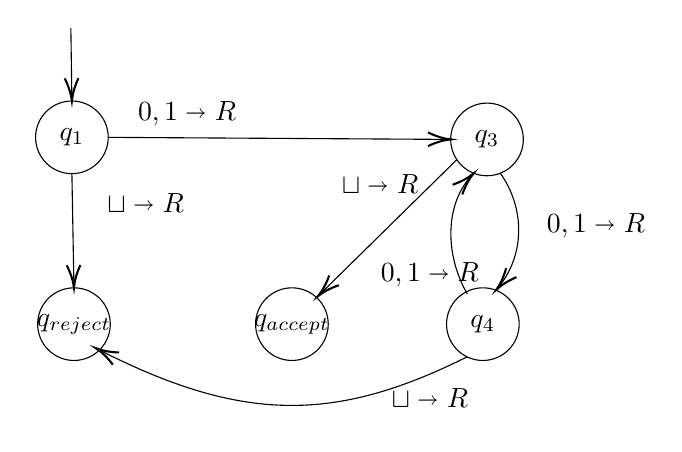
\begin{tikzpicture}[x=0.75pt,y=0.75pt,yscale=-1,xscale=1]
	%uncomment if require: \path (0,242.2857208251953); %set diagram left start at 0, and has height of 242.2857208251953
	
	%Shape: Circle [id:dp8970873053324881] 
	\draw   (204,78) .. controls (204,68.34) and (211.84,60.5) .. (221.5,60.5) .. controls (231.16,60.5) and (239,68.34) .. (239,78) .. controls (239,87.66) and (231.16,95.5) .. (221.5,95.5) .. controls (211.84,95.5) and (204,87.66) .. (204,78) -- cycle ;
	%Shape: Circle [id:dp008553817874642489] 
	\draw   (404,79) .. controls (404,69.34) and (411.84,61.5) .. (421.5,61.5) .. controls (431.16,61.5) and (439,69.34) .. (439,79) .. controls (439,88.66) and (431.16,96.5) .. (421.5,96.5) .. controls (411.84,96.5) and (404,88.66) .. (404,79) -- cycle ;
	%Shape: Circle [id:dp18981812475350313] 
	\draw   (205,168) .. controls (205,158.34) and (212.84,150.5) .. (222.5,150.5) .. controls (232.16,150.5) and (240,158.34) .. (240,168) .. controls (240,177.66) and (232.16,185.5) .. (222.5,185.5) .. controls (212.84,185.5) and (205,177.66) .. (205,168) -- cycle ;
	%Shape: Circle [id:dp25608056185792316] 
	\draw   (402,168) .. controls (402,158.34) and (409.84,150.5) .. (419.5,150.5) .. controls (429.16,150.5) and (437,158.34) .. (437,168) .. controls (437,177.66) and (429.16,185.5) .. (419.5,185.5) .. controls (409.84,185.5) and (402,177.66) .. (402,168) -- cycle ;
	%Straight Lines [id:da43649293419672053] 
	\draw    (221,25.43) -- (221.47,58.5) ;
	\draw [shift={(221.5,60.5)}, rotate = 269.18] [color={rgb, 255:red, 0; green, 0; blue, 0 }  ][line width=0.75]    (10.93,-3.29) .. controls (6.95,-1.4) and (3.31,-0.3) .. (0,0) .. controls (3.31,0.3) and (6.95,1.4) .. (10.93,3.29)   ;
	
	%Straight Lines [id:da5251872130952686] 
	\draw    (221.5,95.5) -- (222.46,148.5) ;
	\draw [shift={(222.5,150.5)}, rotate = 268.96] [color={rgb, 255:red, 0; green, 0; blue, 0 }  ][line width=0.75]    (10.93,-3.29) .. controls (6.95,-1.4) and (3.31,-0.3) .. (0,0) .. controls (3.31,0.3) and (6.95,1.4) .. (10.93,3.29)   ;
	
	%Curve Lines [id:da49256987489536996] 
	\draw    (428,95.43) .. controls (439.64,111.92) and (439.99,134.05) .. (427.22,149.97) ;
	\draw [shift={(426,151.43)}, rotate = 311.19] [color={rgb, 255:red, 0; green, 0; blue, 0 }  ][line width=0.75]    (10.93,-3.29) .. controls (6.95,-1.4) and (3.31,-0.3) .. (0,0) .. controls (3.31,0.3) and (6.95,1.4) .. (10.93,3.29)   ;
	
	%Curve Lines [id:da5559424712444547] 
	\draw    (413.58,96.94) .. controls (401.01,111.17) and (401.38,135.09) .. (412,153.43) ;
	
	\draw [shift={(415,95.43)}, rotate = 135] [color={rgb, 255:red, 0; green, 0; blue, 0 }  ][line width=0.75]    (10.93,-3.29) .. controls (6.95,-1.4) and (3.31,-0.3) .. (0,0) .. controls (3.31,0.3) and (6.95,1.4) .. (10.93,3.29)   ;
	%Straight Lines [id:da2007350951308391] 
	\draw    (239,78) -- (402,78.99) ;
	\draw [shift={(404,79)}, rotate = 180.35] [color={rgb, 255:red, 0; green, 0; blue, 0 }  ][line width=0.75]    (10.93,-3.29) .. controls (6.95,-1.4) and (3.31,-0.3) .. (0,0) .. controls (3.31,0.3) and (6.95,1.4) .. (10.93,3.29)   ;
	
	%Shape: Circle [id:dp6233332615538876] 
	\draw   (310,168) .. controls (310,158.34) and (317.84,150.5) .. (327.5,150.5) .. controls (337.16,150.5) and (345,158.34) .. (345,168) .. controls (345,177.66) and (337.16,185.5) .. (327.5,185.5) .. controls (317.84,185.5) and (310,177.66) .. (310,168) -- cycle ;
	%Straight Lines [id:da13965231887723584] 
	\draw    (407,88.71) -- (341.43,153.17) ;
	\draw [shift={(340,154.57)}, rotate = 315.49] [color={rgb, 255:red, 0; green, 0; blue, 0 }  ][line width=0.75]    (10.93,-3.29) .. controls (6.95,-1.4) and (3.31,-0.3) .. (0,0) .. controls (3.31,0.3) and (6.95,1.4) .. (10.93,3.29)   ;
	
	%Curve Lines [id:da47991408261454205] 
	\draw    (412,183.71) .. controls (348.32,215.55) and (303.45,215.57) .. (234.05,180.11) ;
	\draw [shift={(233,179.57)}, rotate = 387.22] [color={rgb, 255:red, 0; green, 0; blue, 0 }  ][line width=0.75]    (10.93,-3.29) .. controls (6.95,-1.4) and (3.31,-0.3) .. (0,0) .. controls (3.31,0.3) and (6.95,1.4) .. (10.93,3.29)   ;
	
	% Text Node
	\draw (257,109.43) node  [align=left] {$\displaystyle \sqcup \shortrightarrow R$};
	% Text Node
	\draw (474,120.43) node  [align=left] {$\displaystyle 0,1\shortrightarrow R$};
	% Text Node
	\draw (394,144.43) node  [align=left] {$\displaystyle 0,1\shortrightarrow R$};
	% Text Node
	\draw (221.5,78) node  [align=left] {$\displaystyle q_{1}$};
	% Text Node
	\draw (421.5,79) node  [align=left] {$\displaystyle q_{3}$};
	% Text Node
	\draw (419.5,168) node  [align=left] {$\displaystyle q_{4}$};
	% Text Node
	\draw (222.5,168) node  [align=left] {$\displaystyle q_{reject}$};
	% Text Node
	\draw (277,66.43) node  [align=left] {$\displaystyle 0,1\shortrightarrow R$};
	% Text Node
	\draw (370,100.43) node  [align=left] {$\displaystyle \sqcup \shortrightarrow R$};
	% Text Node
	\draw (327.5,168) node  [align=left] {$\displaystyle q_{accept}$};
	% Text Node
	\draw (394,203.43) node  [align=left] {$\displaystyle \sqcup \shortrightarrow R$};
	
	\end{tikzpicture}

Input string 000: 

	\tikzset{every picture/.style={line width=0.75pt}} %set default line width to 0.75pt        
	
	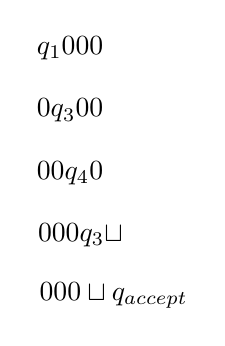
\begin{tikzpicture}[x=0.75pt,y=0.75pt,yscale=-1,xscale=1]
	%uncomment if require: \path (0,184.7142791748047); %set diagram left start at 0, and has height of 184.7142791748047
	
	% Text Node
	\draw (307,43) node  [align=left] {$\displaystyle q_{1} 000$};
	% Text Node
	\draw (307,73) node  [align=left] {$\displaystyle 0q_{3} 00$};
	% Text Node
	\draw (307,103) node  [align=left] {$\displaystyle 00q_{4} 0$};
	% Text Node
	\draw (312,133) node  [align=left] {$\displaystyle 000q_{3} \sqcup $};
	% Text Node
	\draw (328,162) node  [align=left] {$\displaystyle 000\sqcup q_{accept}$};
	
	\end{tikzpicture}

Input string 0000: 

	\tikzset{every picture/.style={line width=0.75pt}} %set default line width to 0.75pt        
	
	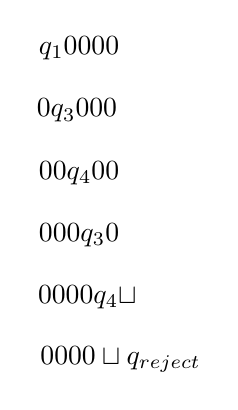
\begin{tikzpicture}[x=0.75pt,y=0.75pt,yscale=-1,xscale=1]
	%uncomment if require: \path (0,300); %set diagram left start at 0, and has height of 300
	
	% Text Node
	\draw (275,64) node  [align=left] {$\displaystyle q_{1} 0000$};
	% Text Node
	\draw (274,94) node  [align=left] {$\displaystyle 0q_{3} 000$};
	% Text Node
	\draw (275,124) node  [align=left] {$\displaystyle 00q_{4} 00$};
	% Text Node
	\draw (275,154) node  [align=left] {$\displaystyle 000q_{3} 0$};
	% Text Node
	\draw (279,184) node  [align=left] {$\displaystyle 0000q_{4} \sqcup $};
	% Text Node
	\draw (295,214) node  [align=left] {$\displaystyle 0000\sqcup q_{reject}$};
	
	\end{tikzpicture}

Modified M2 for detecting even number of 0s: 

	\tikzset{every picture/.style={line width=0.75pt}} %set default line width to 0.75pt        
	
	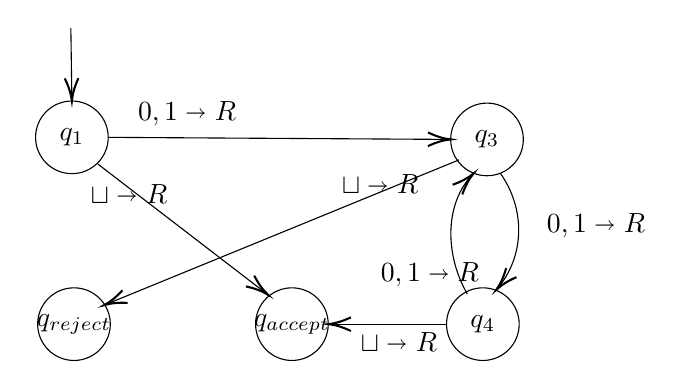
\begin{tikzpicture}[x=0.75pt,y=0.75pt,yscale=-1,xscale=1]
	%uncomment if require: \path (0,253.14285278320312); %set diagram left start at 0, and has height of 253.14285278320312
	
	%Shape: Circle [id:dp8712066356771144] 
	\draw   (204,89) .. controls (204,79.34) and (211.84,71.5) .. (221.5,71.5) .. controls (231.16,71.5) and (239,79.34) .. (239,89) .. controls (239,98.66) and (231.16,106.5) .. (221.5,106.5) .. controls (211.84,106.5) and (204,98.66) .. (204,89) -- cycle ;
	%Shape: Circle [id:dp4941071822022003] 
	\draw   (404,90) .. controls (404,80.34) and (411.84,72.5) .. (421.5,72.5) .. controls (431.16,72.5) and (439,80.34) .. (439,90) .. controls (439,99.66) and (431.16,107.5) .. (421.5,107.5) .. controls (411.84,107.5) and (404,99.66) .. (404,90) -- cycle ;
	%Shape: Circle [id:dp49452005321317993] 
	\draw   (205,179) .. controls (205,169.34) and (212.84,161.5) .. (222.5,161.5) .. controls (232.16,161.5) and (240,169.34) .. (240,179) .. controls (240,188.66) and (232.16,196.5) .. (222.5,196.5) .. controls (212.84,196.5) and (205,188.66) .. (205,179) -- cycle ;
	%Shape: Circle [id:dp5674759827725786] 
	\draw   (402,179) .. controls (402,169.34) and (409.84,161.5) .. (419.5,161.5) .. controls (429.16,161.5) and (437,169.34) .. (437,179) .. controls (437,188.66) and (429.16,196.5) .. (419.5,196.5) .. controls (409.84,196.5) and (402,188.66) .. (402,179) -- cycle ;
	%Straight Lines [id:da020043005699736938] 
	\draw    (221,36.43) -- (221.47,69.5) ;
	\draw [shift={(221.5,71.5)}, rotate = 269.18] [color={rgb, 255:red, 0; green, 0; blue, 0 }  ][line width=0.75]    (10.93,-3.29) .. controls (6.95,-1.4) and (3.31,-0.3) .. (0,0) .. controls (3.31,0.3) and (6.95,1.4) .. (10.93,3.29)   ;
	
	%Straight Lines [id:da6541314362892807] 
	\draw    (234,101.86) -- (314.41,163.64) ;
	\draw [shift={(316,164.86)}, rotate = 217.53] [color={rgb, 255:red, 0; green, 0; blue, 0 }  ][line width=0.75]    (10.93,-3.29) .. controls (6.95,-1.4) and (3.31,-0.3) .. (0,0) .. controls (3.31,0.3) and (6.95,1.4) .. (10.93,3.29)   ;
	
	%Curve Lines [id:da39062413650936767] 
	\draw    (428,106.43) .. controls (439.64,122.92) and (439.99,145.05) .. (427.22,160.97) ;
	\draw [shift={(426,162.43)}, rotate = 311.19] [color={rgb, 255:red, 0; green, 0; blue, 0 }  ][line width=0.75]    (10.93,-3.29) .. controls (6.95,-1.4) and (3.31,-0.3) .. (0,0) .. controls (3.31,0.3) and (6.95,1.4) .. (10.93,3.29)   ;
	
	%Curve Lines [id:da8218971597623406] 
	\draw    (413.58,107.94) .. controls (401.01,122.17) and (401.38,146.09) .. (412,164.43) ;
	
	\draw [shift={(415,106.43)}, rotate = 135] [color={rgb, 255:red, 0; green, 0; blue, 0 }  ][line width=0.75]    (10.93,-3.29) .. controls (6.95,-1.4) and (3.31,-0.3) .. (0,0) .. controls (3.31,0.3) and (6.95,1.4) .. (10.93,3.29)   ;
	%Straight Lines [id:da18289168145848866] 
	\draw    (239,89) -- (402,89.99) ;
	\draw [shift={(404,90)}, rotate = 180.35] [color={rgb, 255:red, 0; green, 0; blue, 0 }  ][line width=0.75]    (10.93,-3.29) .. controls (6.95,-1.4) and (3.31,-0.3) .. (0,0) .. controls (3.31,0.3) and (6.95,1.4) .. (10.93,3.29)   ;
	
	%Shape: Circle [id:dp04024660167443028] 
	\draw   (310,179) .. controls (310,169.34) and (317.84,161.5) .. (327.5,161.5) .. controls (337.16,161.5) and (345,169.34) .. (345,179) .. controls (345,188.66) and (337.16,196.5) .. (327.5,196.5) .. controls (317.84,196.5) and (310,188.66) .. (310,179) -- cycle ;
	%Straight Lines [id:da43553808885026535] 
	\draw    (402,179) -- (347,179) ;
	\draw [shift={(345,179)}, rotate = 360] [color={rgb, 255:red, 0; green, 0; blue, 0 }  ][line width=0.75]    (10.93,-3.29) .. controls (6.95,-1.4) and (3.31,-0.3) .. (0,0) .. controls (3.31,0.3) and (6.95,1.4) .. (10.93,3.29)   ;
	
	%Straight Lines [id:da40594825659318245] 
	\draw    (408,99.86) -- (238.85,169.1) ;
	\draw [shift={(237,169.86)}, rotate = 337.74] [color={rgb, 255:red, 0; green, 0; blue, 0 }  ][line width=0.75]    (10.93,-3.29) .. controls (6.95,-1.4) and (3.31,-0.3) .. (0,0) .. controls (3.31,0.3) and (6.95,1.4) .. (10.93,3.29)   ;
	
	% Text Node
	\draw (249,116.43) node  [align=left] {$\displaystyle \sqcup \shortrightarrow R$};
	% Text Node
	\draw (474,131.43) node  [align=left] {$\displaystyle 0,1\shortrightarrow R$};
	% Text Node
	\draw (394,155.43) node  [align=left] {$\displaystyle 0,1\shortrightarrow R$};
	% Text Node
	\draw (221.5,89) node  [align=left] {$\displaystyle q_{1}$};
	% Text Node
	\draw (421.5,90) node  [align=left] {$\displaystyle q_{3}$};
	% Text Node
	\draw (419.5,179) node  [align=left] {$\displaystyle q_{4}$};
	% Text Node
	\draw (222.5,179) node  [align=left] {$\displaystyle q_{reject}$};
	% Text Node
	\draw (277,77.43) node  [align=left] {$\displaystyle 0,1\shortrightarrow R$};
	% Text Node
	\draw (370,111.43) node  [align=left] {$\displaystyle \sqcup \shortrightarrow R$};
	% Text Node
	\draw (327.5,179) node  [align=left] {$\displaystyle q_{accept}$};
	% Text Node
	\draw (379,187.43) node  [align=left] {$\displaystyle \sqcup \shortrightarrow R$};
	
	\end{tikzpicture}

Input string 000: 	

	\tikzset{every picture/.style={line width=0.75pt}} %set default line width to 0.75pt        
	
	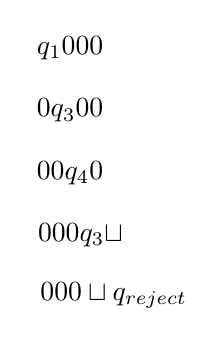
\begin{tikzpicture}[x=0.75pt,y=0.75pt,yscale=-1,xscale=1]
	%uncomment if require: \path (0,184.7142791748047); %set diagram left start at 0, and has height of 184.7142791748047
	
	% Text Node
	\draw (307,43) node  [align=left] {$\displaystyle q_{1} 000$};
	% Text Node
	\draw (307,73) node  [align=left] {$\displaystyle 0q_{3} 00$};
	% Text Node
	\draw (307,103) node  [align=left] {$\displaystyle 00q_{4} 0$};
	% Text Node
	\draw (312,133) node  [align=left] {$\displaystyle 000q_{3} \sqcup $};
	% Text Node
	\draw (328,162) node  [align=left] {$\displaystyle 000\sqcup q_{reject}$};
	
	\end{tikzpicture}

Input string 0000: 

	\tikzset{every picture/.style={line width=0.75pt}} %set default line width to 0.75pt        
	
	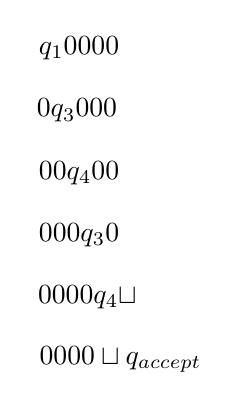
\begin{tikzpicture}[x=0.75pt,y=0.75pt,yscale=-1,xscale=1]
	%uncomment if require: \path (0,300); %set diagram left start at 0, and has height of 300
	
	% Text Node
	\draw (275,64) node  [align=left] {$\displaystyle q_{1} 0000$};
	% Text Node
	\draw (274,94) node  [align=left] {$\displaystyle 0q_{3} 000$};
	% Text Node
	\draw (275,124) node  [align=left] {$\displaystyle 00q_{4} 00$};
	% Text Node
	\draw (275,154) node  [align=left] {$\displaystyle 000q_{3} 0$};
	% Text Node
	\draw (279,184) node  [align=left] {$\displaystyle 0000q_{4} \sqcup $};
	% Text Node
	\draw (295,214) node  [align=left] {$\displaystyle 0000\sqcup q_{accept}$};
	
	\end{tikzpicture}

\end{document}